% Copyright (C) 2022 - Joseph Muré

\documentclass[aspectratio=169]{beamer}

%\setbeameroption{hide notes}
%\setbeameroption{show notes}
%\setbeameroption{show only notes}

% Copyright (C) 2012 - EDF R&D - Michael Baudin

% To highlight source code
\usepackage{listings}
\definecolor{darkgreen}{rgb}{0,0.5,0}
\definecolor{violet}{rgb}{0.5,0,1}

\usepackage{lmodern}% http://ctan.org/pkg/lm

\usetheme{Montpellier}
\setbeamertemplate{navigation symbols}{} % Remove navigation
\useoutertheme{infolines}

\usepackage[utf8]{inputenc}
\usepackage[T1]{fontenc}

\usepackage{graphicx}
\unitlength=1cm
\graphicspath{{./figures/}}

\usepackage{hyperref}
\hypersetup{colorlinks=true, linkcolor=blue, linktocpage, urlcolor=blue}

\def\bx{{\bf x}}
\def\RR{\mathbb{R}}

\newcommand{\pyvar}[1]{\texttt{#1}}

\def \ot {OpenTURNS}

\definecolor{codegreen}{rgb}{0,0.6,0}
\definecolor{codegray}{rgb}{0.5,0.5,0.5}
\definecolor{codepurple}{rgb}{0.58,0,0.82}
\definecolor{backcolour}{rgb}{0.95,0.95,0.92}
\lstdefinestyle{mystyle}{
  backgroundcolor=\color{backcolour},   commentstyle=\color{codegreen},
  keywordstyle=\color{magenta},
  numberstyle=\tiny\color{codegray},
  stringstyle=\color{codepurple},
  basicstyle=\ttfamily\tiny,
  breakatwhitespace=false,         
  breaklines=true,                 
  captionpos=b,                    
  keepspaces=true,                 
  numbers=left,                    
  numbersep=5pt,                  
  showspaces=false,                
  showstringspaces=false,
  showtabs=false,                  
  tabsize=1,
  numbers=none
}

\lstset{style=mystyle, language=python}


\usepackage{tikz}
\usetikzlibrary{positioning}

\renewcommand{\footnotesize}{\tiny}

\title[OpenTURNS]{Overview of OpenTURNS, its new features and its graphical user interface}

\author[J. Pelamatti]{
The OpenTURNS Dev Team \\ \vspace{10pt} \small{Presented by J. Pelamatti \inst{1}
}}

\institute[EDF]{
\inst{1} EDF R\&D. 6, quai Watier, 78401, Chatou - France, julien.pelamatti@edf.fr  %
}

\date[]{June 14th 2023, UNCECOMP, Athens, Greece}

\definecolor{codegreen}{rgb}{0,0.6,0}
\definecolor{codegray}{rgb}{0.5,0.5,0.5}
\definecolor{codepurple}{rgb}{0.58,0,0.82}
\definecolor{backcolour}{rgb}{0.95,0.95,0.92}
\lstdefinestyle{mystyle}{
  backgroundcolor=\color{backcolour},   commentstyle=\color{codegreen},
  keywordstyle=\color{magenta},
  numberstyle=\tiny\color{codegray},
  stringstyle=\color{codepurple},
  basicstyle=\ttfamily\tiny,
  breakatwhitespace=false,         
  breaklines=true,                 
  captionpos=b,                    
  keepspaces=true,                 
  numbers=left,                    
  numbersep=5pt,                  
  showspaces=false,                
  showstringspaces=false,
  showtabs=false,                  
  tabsize=1,
  numbers=none
}

\lstset{style=mystyle, language=python}

%%%%%%%%%%%%%%%%%%%%%%%%%%%%%%%%%%%%%%%%%%%%%%%%%%%%%%%%%%%%%%%%%%%%%%%%%%%%%

  \begin{document}

%%%%%%%%%%%%%%%%%%%%%%%%%%%%%%%%%%%%%%%%%%%%%%%%%%%%%%%%%%%%%%%%%%%%%%%%%%%%%

  \begin{frame}
  \titlepage
  
  \begin{columns}
    \column{0.2\textwidth}
  \begin{center}

\includegraphics[height=0.15\textheight]{figures/edf.jpg}
\end{center}	
    \column{0.2\textwidth}
  \begin{center}

\includegraphics[height=0.11\textheight]{figures/LogoAirbus.png}
\end{center}
    \column{0.2\textwidth}
  \begin{center}

\includegraphics[height=0.15\textheight]{figures/logo_phimeca.png}
\end{center}
    \column{0.2\textwidth}
  \begin{center}

\includegraphics[height=0.15\textheight]{figures/logo_Imacs.png}
\end{center}
    \column{0.2\textwidth}
  \begin{center}

\includegraphics[height=0.15\textheight]{figures/logo_ONERA.jpg}
\end{center}
  \end{columns}

  \end{frame}


%%%%%%%%%%%%%%%%%%%%%%%%%%%%%%%%%%%%%%%%%%%%%%%%%%%%%%%%%%%%%%%%%%%%%%%%%%%%%

% \begin{frame}
% \frametitle{Contents}
% \tableofcontents
% \end{frame}

%%%%%%%%%%%%%%%%%%%%%%%%%%%%%%%%%%%%%%%%%%%%%%%%%%%%%%%%%%%%%%%%%%%%%%%%%%%%%
\section{OpenTURNS Overview}

%%%%%%%%%%%%%%%%%%%%%%%%%%%%%%%%%%%%%%%%%%%%%%%%%%%%%%%%%%%%%%%%%%%%%%%%%%%%%

\begin{frame}
\frametitle{OpenTURNS: \url{www.openturns.org}}


    \begin{center}
    
\includegraphics[width=0.65\textwidth]{figures/OT.png}
    \end{center}
	
\begin{itemize}
\item Multivariate probabilistic modeling including complex dependencies
\item Numerical tools dedicated to the treatment of uncertainties
\item Generic coupling to any type of physical model
\item Open source, LGPL licensed, C++ library with a Python interface
\end{itemize}


\end{frame}

\note{
OpenTURNS is software for uncertainty quantification, uncertainty propagation,
sensitivity analysis and metamodeling. 

It is available with the open source LGPL licence on Linux, Windows and macOS.

In order to use OpenTURNS, you can use directly the C++ library, or 
program your Python scripts. 
}
%%%%%%%%%%%%%%%%%%%%%%%%%%%%%%%%%%%%%%%%%%%%%%%%%%%%%%%%%%%%%%%%%%%%%%%%%%%%%

\begin{frame}
\frametitle{OpenTURNS: \url{www.openturns.org}}

\begin{center}
   \begin{tabular}{ccccc}
   
\includegraphics[width=0.07\textwidth]{figures/logoEDF_Anne.png}&
   
\includegraphics[width=0.12\textwidth]{figures/LogoAirbus.png}&
   
\includegraphics[width=0.12\textwidth]{figures/logo_phimeca.png}&
   
\includegraphics[width=0.12\textwidth]{figures/logo_Imacs.png}
   
\includegraphics[width=0.30\textwidth]{figures/logo_ONERA.jpg}&
   \end{tabular}
\end{center}

\vspace*{0.05cm}
\begin{itemize}
\item Linux, Windows, macOS, Android
\item First release: 2007
\item 5 full time developers
\item $\approx $ 1 000 000 Total Conda downloads since 2016, $\approx $  5000 monthly pipy downloads
\item Project size: 800  classes, more than 6000 services
\item Available in Debian \emph{Bookworm}, Ubuntu, \ldots
\end{itemize}


\end{frame}

%%%%%%%%%%%%%%%%%%%%%%%%%%%%%%%%%%%%%%%%%%%%%%%%%%%%%%%%%%%%%%%%%%%%%%%%%%%%%

\begin{frame}[containsverbatim]
  \frametitle{OpenTURNS: content}
  
  \begin{scriptsize}
  
  \begin{minipage}[t]{0.33\textwidth}
  \begin{itemize}
  \item Data analysis
  \begin{itemize}
  \tiny
  \item Parametric Distribution fitting
  \item Non-parametric Distribution fitting
  \item Statistical tests
  \item Estimate dependency and copulas
  \item Estimate stochastic processes
  \end{itemize}
  \end{itemize}
  \end{minipage}%
  \begin{minipage}[t]{0.33\textwidth}
  \begin{itemize}
  \item Probabilistic modeling
  \begin{itemize}
  \tiny
  \item Dependence modeling
  \item Univariate distributions
  \item Multivariate distributions
  \item Copulas
  \item Processes 
  \item Covariance kernels
  \end{itemize}
  \end{itemize}
  \end{minipage}%
  \begin{minipage}[t]{0.33\textwidth}
  \begin{itemize}
  \item Surrogate models
  \begin{itemize}
  \tiny
  \item Linear regression
  \item Polynomial chaos expansion
  \item Gaussian  process regression
  \item Spectral methods
  \item Low rank tensors
  \item Fields metamodel
  \end{itemize}
  \end{itemize}
  \end{minipage}
  
  \vspace{20pt}  
  
  \begin{minipage}[t]{0.33\textwidth}
  \begin{itemize}
  \item Reliability, sensitivity
  \begin{itemize}
  \tiny
  \item Sampling methods
  \item Approximation methods
  \item Sensitivity analysis
  \item Design of experiments
  \end{itemize}
  \end{itemize}
  \end{minipage}%
  \begin{minipage}[t]{0.33\textwidth}
  \begin{itemize}
  \item Calibration
  \begin{itemize}
  \tiny
  \item Least squares calibration
  \item Gaussian calibration
  \item Bayesian calibration
  \end{itemize}
  \end{itemize}
  \end{minipage}%
  \begin{minipage}[t]{0.33\textwidth}
  \begin{itemize}
  \item Numerical methods
  \begin{itemize}
  \tiny
  \item Optimization
  \item Integration
  \item Least squares 
  \item Meshing
  \item Coupling with external codes
  \end{itemize}
  \end{itemize}
  \end{minipage}
  \end{scriptsize}

  \begin{tabular}{@{}c@{}c@{}c@{}c@{}c@{}}
  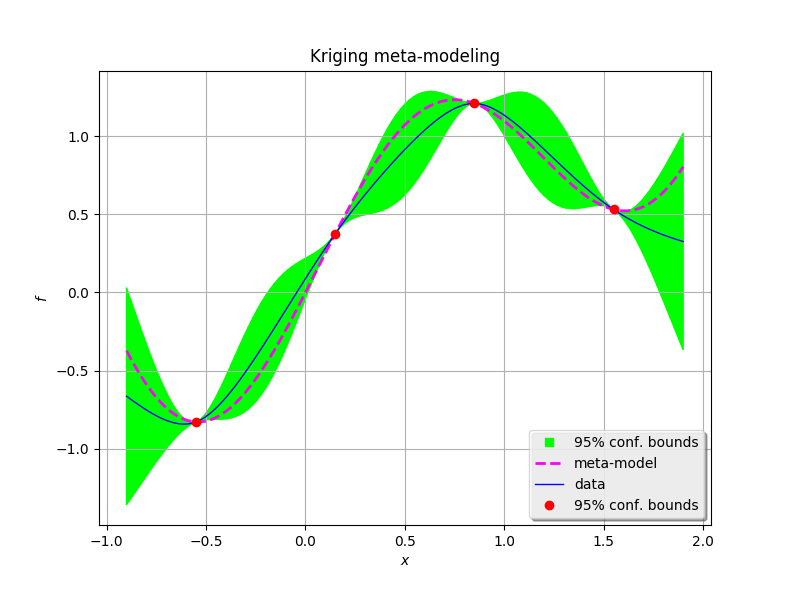
\includegraphics[width=0.2\textwidth]{figures/plot_kriging.png}&
  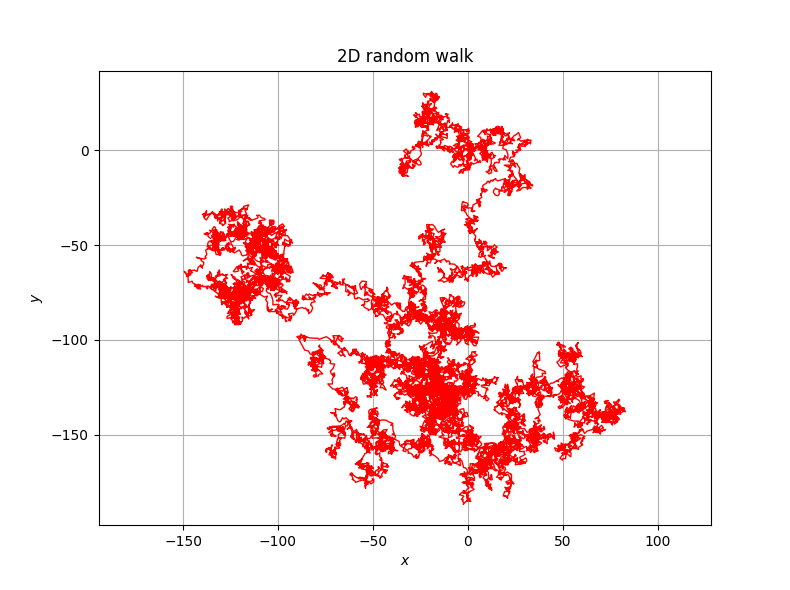
\includegraphics[width=0.2\textwidth]{figures/plot_random_walk.png}&
  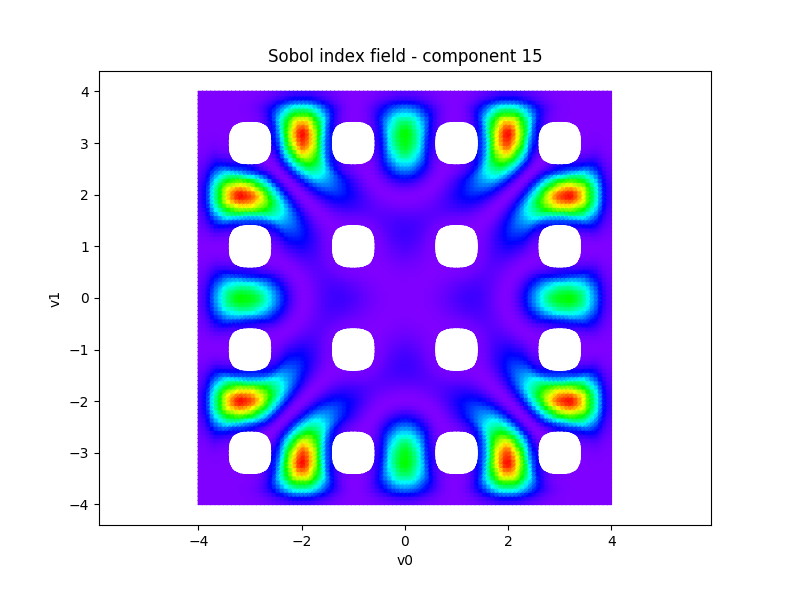
\includegraphics[width=0.2\textwidth]{figures/plot_sobol_field.png}&
  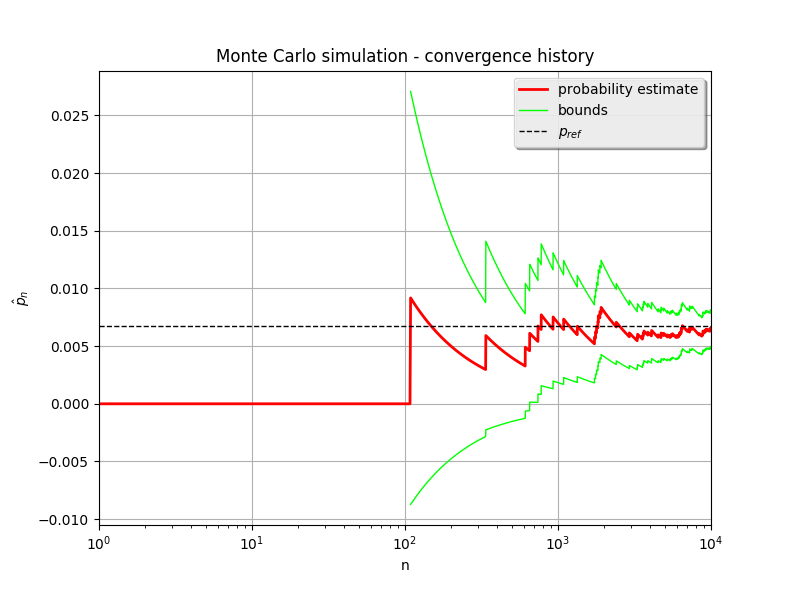
\includegraphics[width=0.2\textwidth]{figures/plot_monte_carlo.png}&
  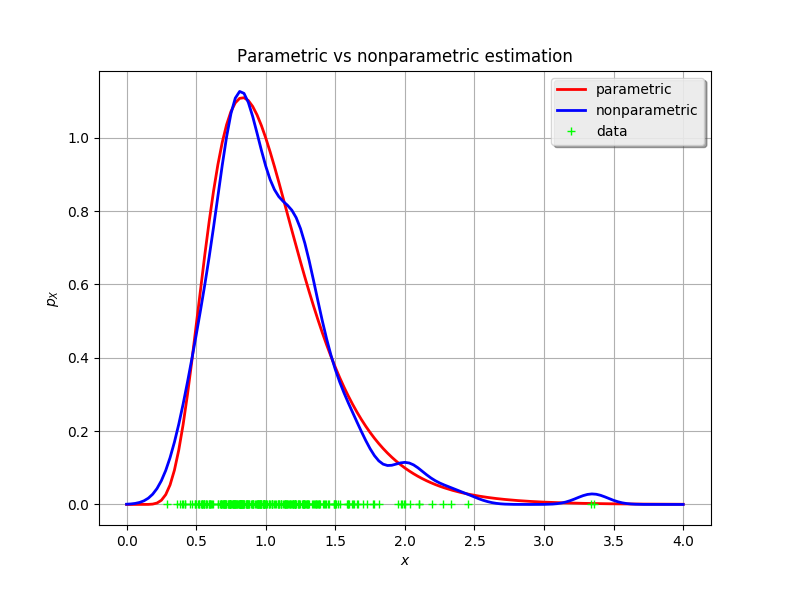
\includegraphics[width=0.2\textwidth]{figures/plot_distribution_fitting.png}
  \end{tabular}
\end{frame}
  
%%%%%%%%%%%%%%%%%%%%%%%%%%%%%%%%%%%%%%%%%%%%%%%%%%%%%%%%%%%%%%%%%%%%%%%%%%%%%

\begin{frame}[containsverbatim]
  \frametitle{OpenTURNS: documentation}
  
  
  \begin{columns}
  	\vspace{10pt}
      \column{0.5\textwidth}
  
  \vspace{-30pt}
      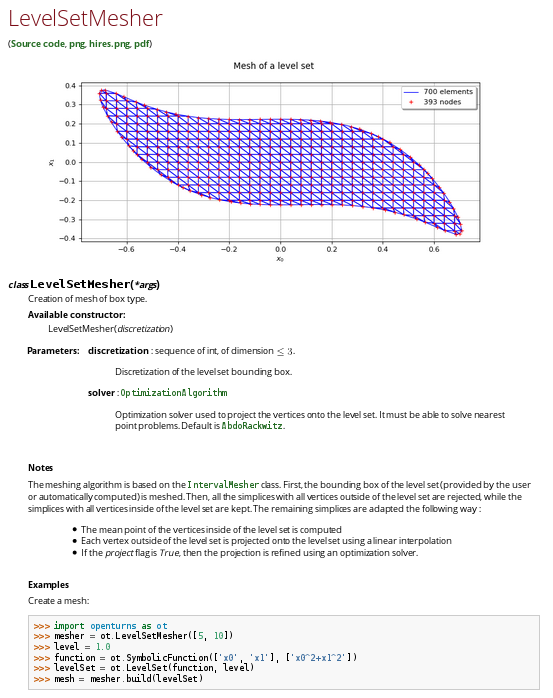
\includegraphics[width=0.7\textwidth]{figures/exClasses.png}
  
      \column{0.5\textwidth}
      
      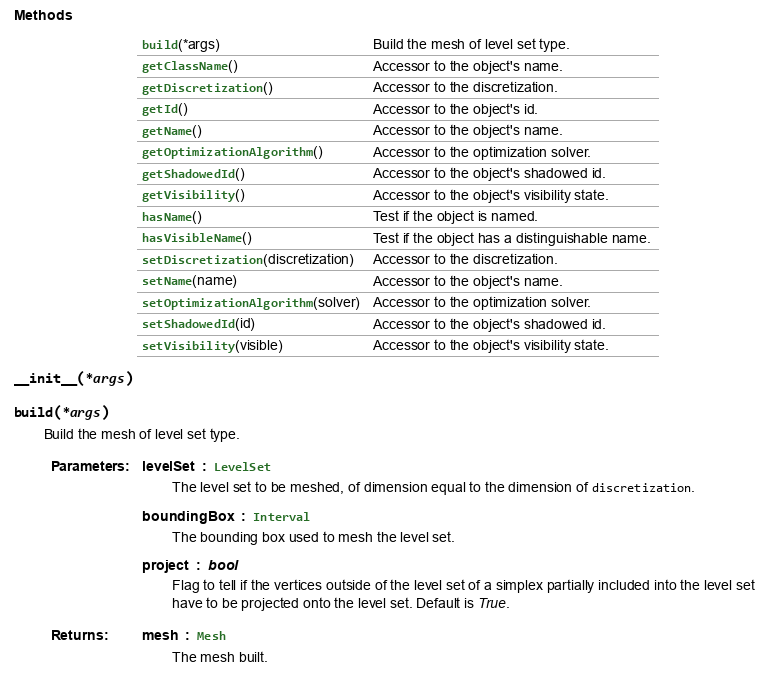
\includegraphics[width=0.6\textwidth]{figures/exClasses2.png}
  
    \scriptsize{

    \begin{itemize}
    \item \underline{Content}: 
    \begin{itemize}
    \item Programming interface (API)
    \item Examples
    \item Theory
    \end{itemize}
    \item \emph{All} classes and methods 
    are documented, partly automatically.
    \item Examples and unit tests are automatically run at \emph{each} code update 
    \end{itemize}
      }
  \end{columns}
  

\end{frame}
  
%%%%%%%%%%%%%%%%%%%%%%%%%%%%%%%%%%%%%%%%%%%%%%%%%%%%%%%%%%%%%%%%%%%%%%%%%%%%%

\begin{frame}[containsverbatim]
  \frametitle{OpenTURNS: practical use}
  
  \small
  \begin{itemize}
  \item Compatibility with several popular python packages
  \begin{itemize}
  \scriptsize
  \item Numpy
  \item Scipy
  \item Matplotlib
  \item Scikit-learn
  \item Pandas
  \end{itemize}
  \vspace{10pt}
  \item Parallel computational with shared memory (TBB)
  \vspace{10pt}
  \item Optimized linear algebra with LAPACK and BLAS 
  \vspace{10pt}
  \item Possibility to interface with a computation cluster
  \vspace{10pt}
  \item Focused towards handling numerical data
  \vspace{10pt}
  \item Installation through conda, pip, packages for various Linux distros and source code
  \end{itemize}
\end{frame}
  


%%%%%%%%%%%%%%%%%%%%%%%%%%%%%%%%%%%%%%%%%%%%%%%%%%%%%%%%%%%%%%%%%%%%%%%%%%%%%%

\begin{frame}[containsverbatim]
\frametitle{Probabilistic modeling}

\scriptsize

\underline{Random variables distributions}: 

\tiny 


\begin{minipage}[t]{0.5\textwidth}

Q: Gumbel(scale=558, mode=1013)>0

    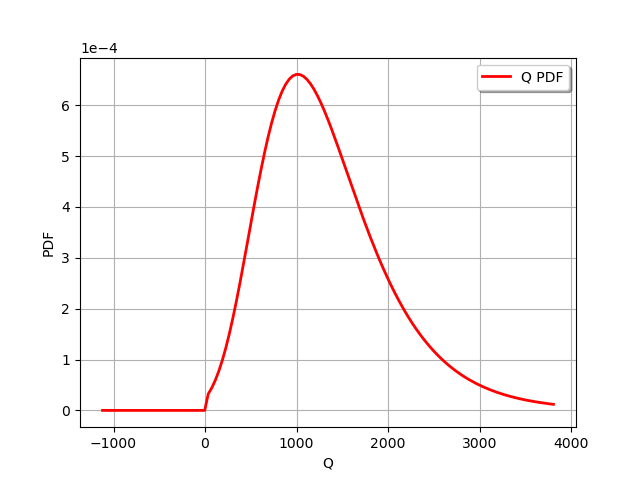
\includegraphics[width=.45\textwidth]{figures/Q.png}
    
\tiny
\begin{lstlisting}[language=Python]
Dist = ot.Gumbel(558,1013)
Q = ot.TruncatedDistribution(Dist, 0.,
ot.TruncatedDistribution.LOWER)
\end{lstlisting}

\end{minipage}%
\begin{minipage}[t]{0.5\textwidth}

Ks: Normal(mean=30, std=7.5)>0

    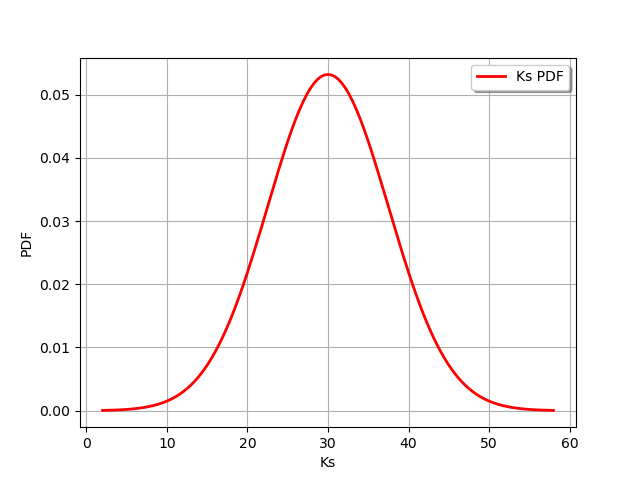
\includegraphics[width=.45\textwidth]{figures/Ks.png}
    
    \tiny
\begin{lstlisting}[language=Python]
Dist = ot.Normal(30.,7.5)
Ks = ot.TruncatedDistribution(Dist, 0., ot.TruncatedDistribution.LOWER)

\end{lstlisting}

\end{minipage}
\begin{minipage}[t]{0.5\textwidth}

Zv: Uniform(min=49, max=51)

    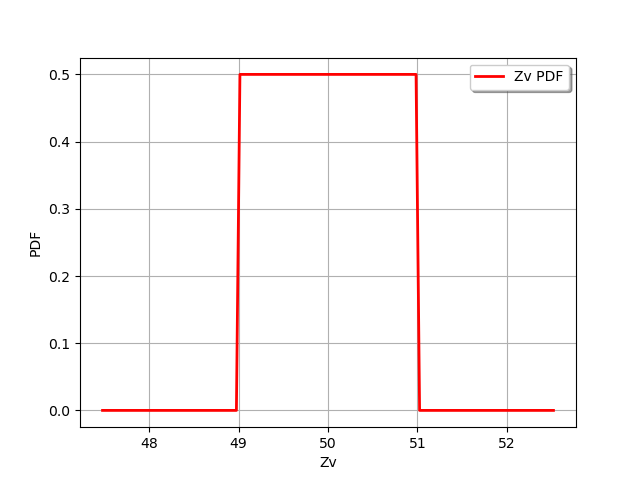
\includegraphics[width=.45\textwidth]{figures/Zv.png}
    
\end{minipage}%
\begin{minipage}[t]{0.5\textwidth}

Zm: Uniform(min=54, max=56)

    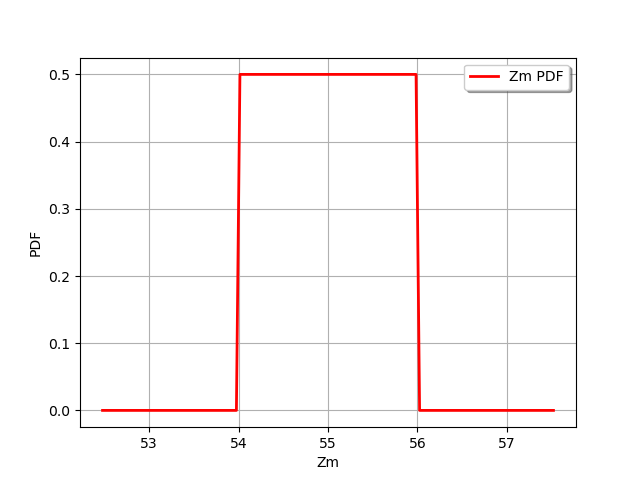
\includegraphics[width=.45\textwidth]{figures/Zm.png}
    
\end{minipage}%

\end{frame}


% %%%%%%%%%%%%%%%%%%%%%%%%%%%%%%%%%%%%%%%%%%%%%%%%%%%%%%%%%%%%%%%%%%%%%%%%%%%%%

\begin{frame}[containsverbatim]
\frametitle{Design of experiments}

\scriptsize{

\begin{itemize}
\item  Different Design of experiment types are available
\item We consider a 2-dimensional distribution with the following marginals: 
\begin{itemize}
\tiny
\item Gumbel(min = -1, max = 1)
\item Truncated normal (mean = 0, std = 1, min = -2, max = 2)
\end{itemize}
\end{itemize}

\begin{columns}
    \column{0.5\textwidth}

\underline{Marginals}

    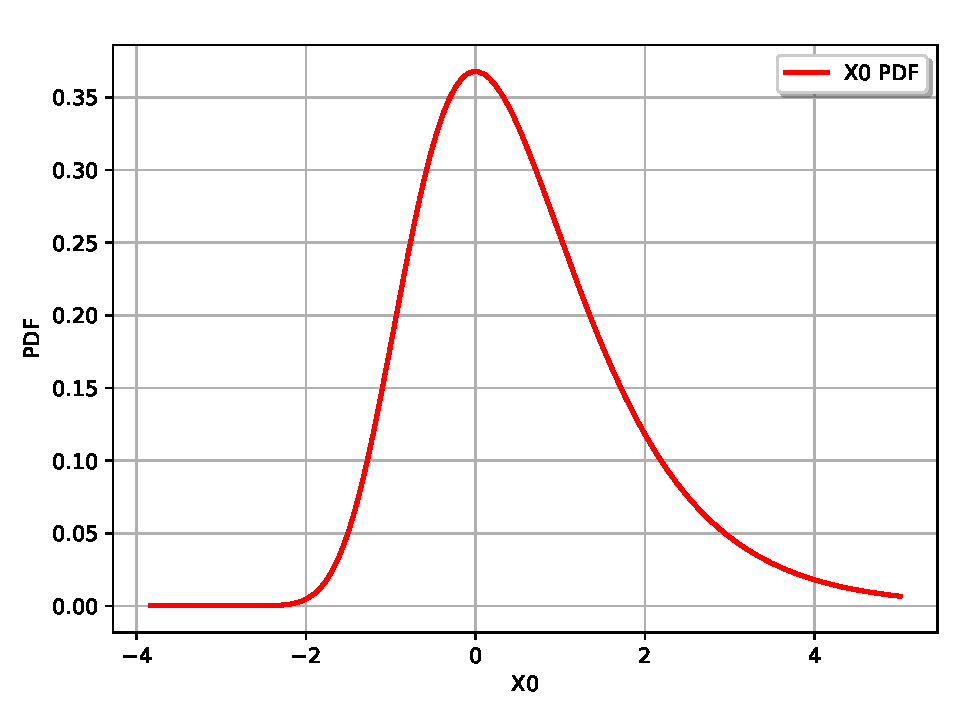
\includegraphics[width=.45\textwidth]{figures/Marg1.pdf}

    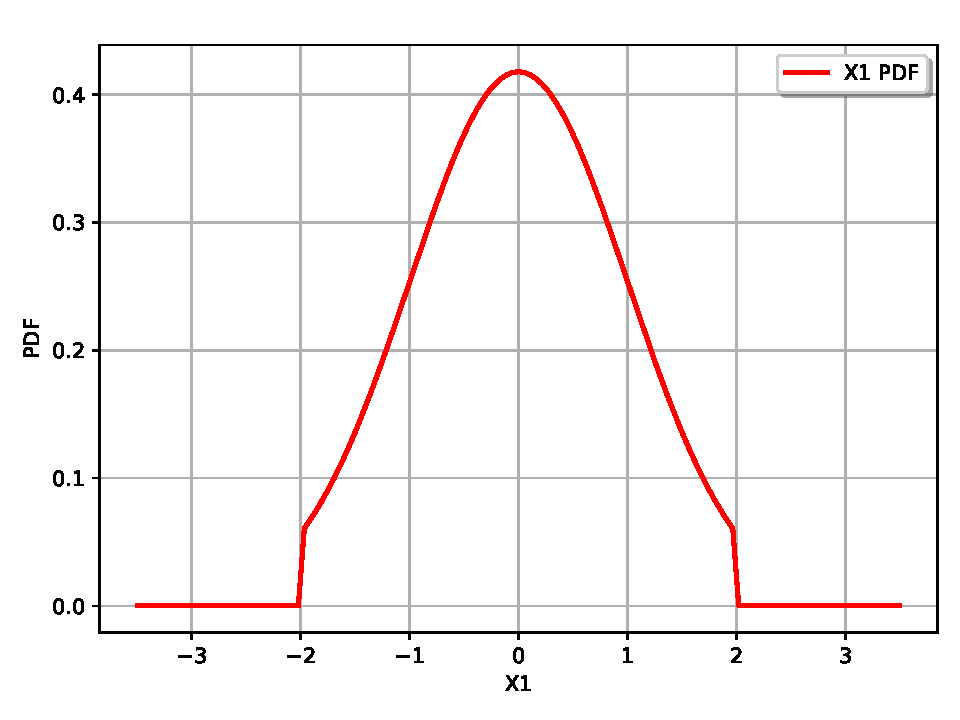
\includegraphics[width=.45\textwidth]{figures/Marg2.pdf}


    \column{0.5\textwidth}
    
\underline{Joint distributions}

    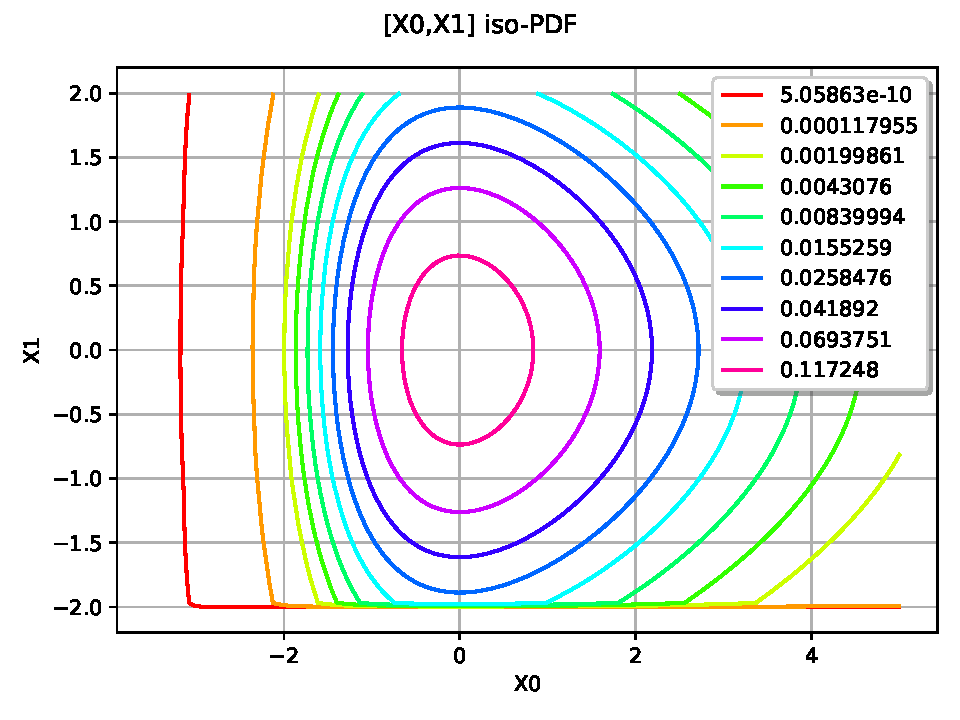
\includegraphics[width=1\textwidth]{figures/Dist.pdf}

	
\end{columns}

}

\end{frame}


% %%%%%%%%%%%%%%%%%%%%%%%%%%%%%%%%%%%%%%%%%%%%%%%%%%%%%%%%%%%%%%%%%%%%%%%%%%%%%

\begin{frame}[containsverbatim]
\frametitle{Beyond independent marginals: Copulas}

\begin{minipage}[t]{0.5\textwidth}
    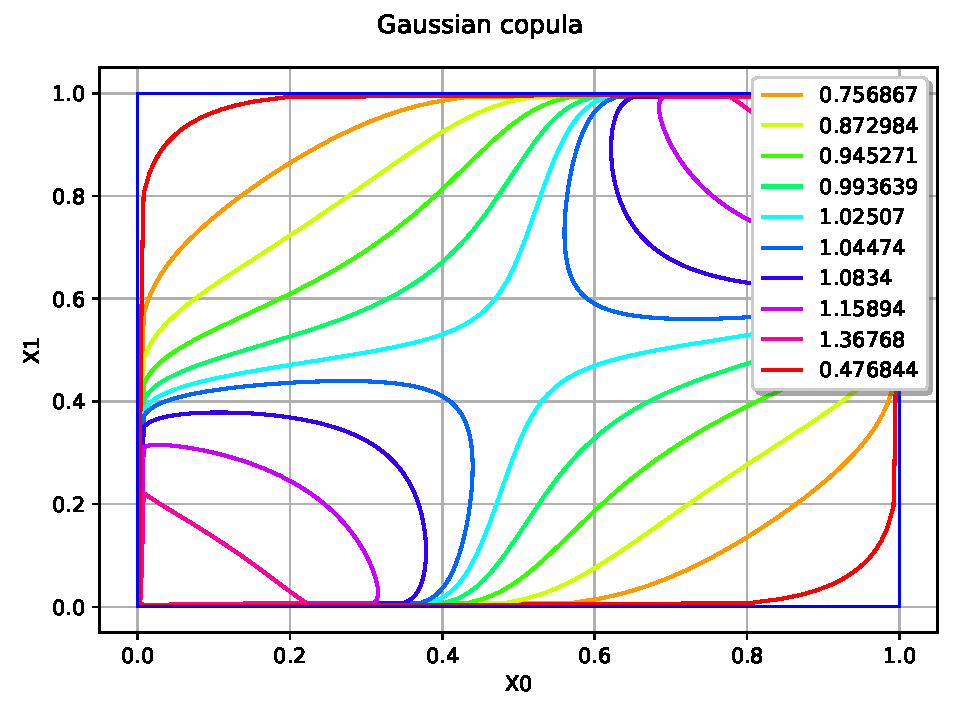
\includegraphics[width=.65\textwidth]{figures/Copula1.pdf}

\end{minipage}%
\begin{minipage}[t]{0.5\textwidth}
    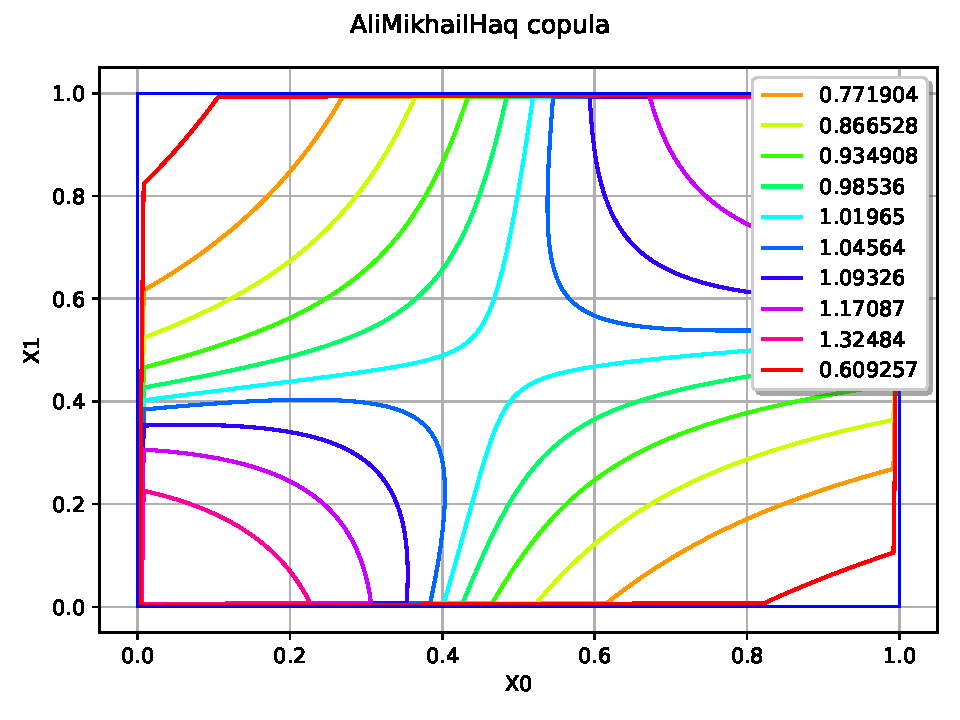
\includegraphics[width=.65\textwidth]{figures/Copula2.pdf}

\end{minipage}
\begin{minipage}[t]{0.5\textwidth}
    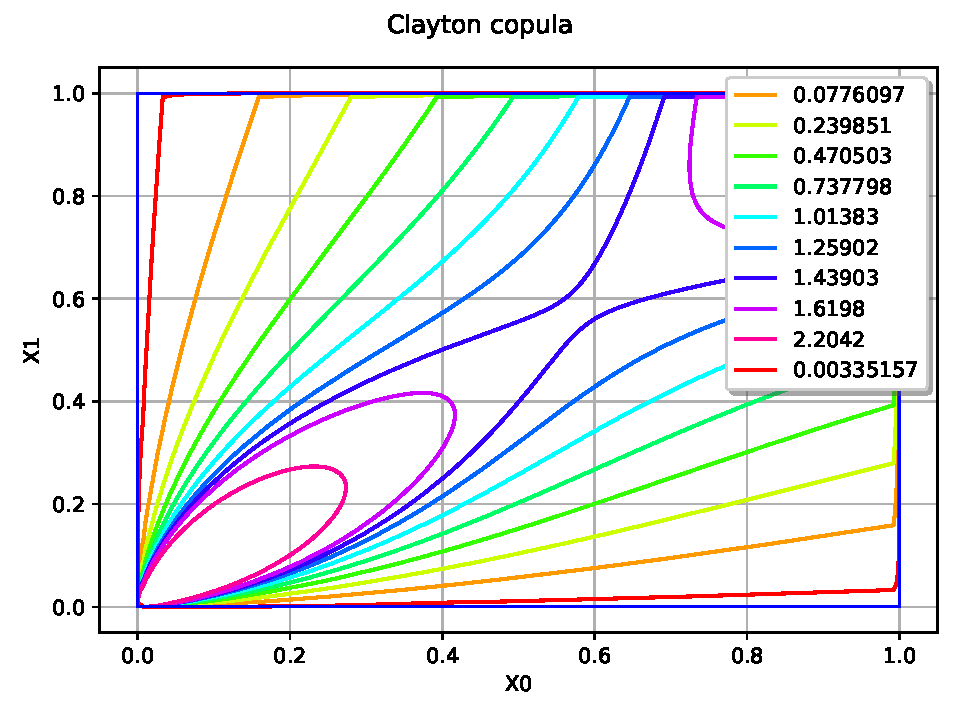
\includegraphics[width=.65\textwidth]{figures/Copula3.pdf}

\end{minipage}%
\begin{minipage}[t]{0.5\textwidth}
    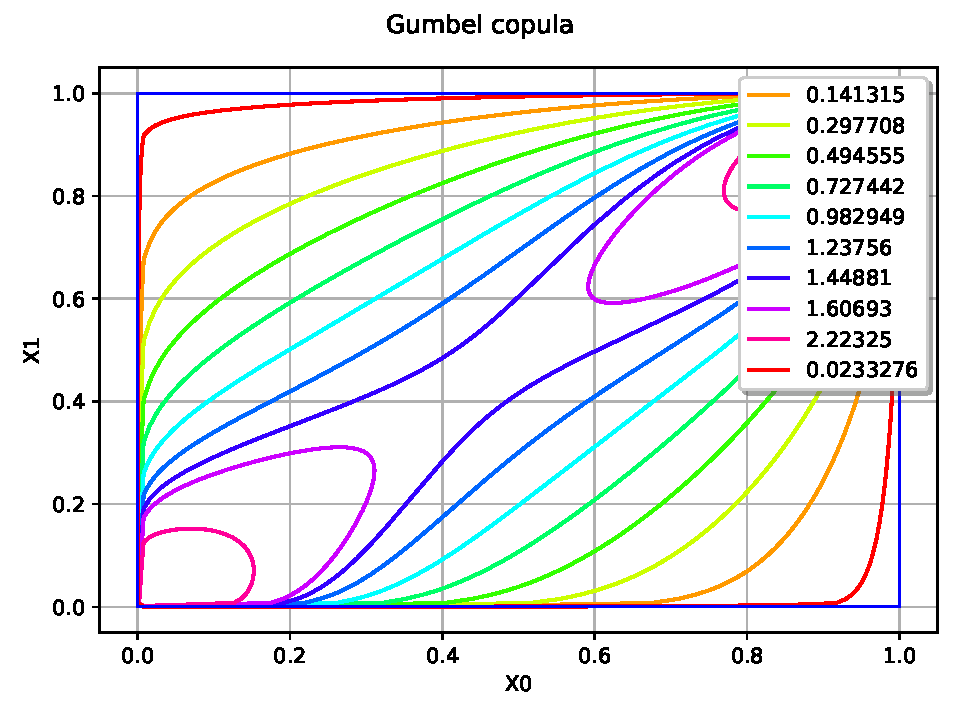
\includegraphics[width=.65\textwidth]{figures/Copula4.pdf}

\end{minipage}

\end{frame}


% %%%%%%%%%%%%%%%%%%%%%%%%%%%%%%%%%%%%%%%%%%%%%%%%%%%%%%%%%%%%%%%%%%%%%%%%%%%%%

\begin{frame}[containsverbatim]
\frametitle{Composing marginal distributions and copulas}

\begin{columns}
    \column{0.5\textwidth}

\begin{minipage}[t]{1.\textwidth}
    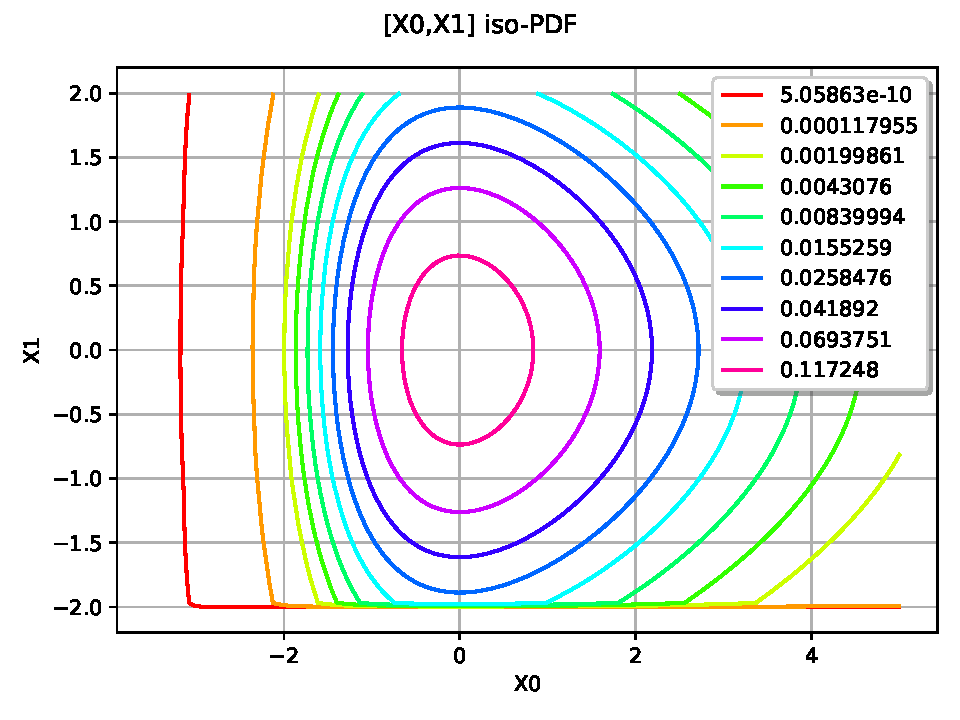
\includegraphics[width=.6\textwidth]{figures/Dist.pdf}

\end{minipage}

\begin{minipage}[t]{1.\textwidth}
    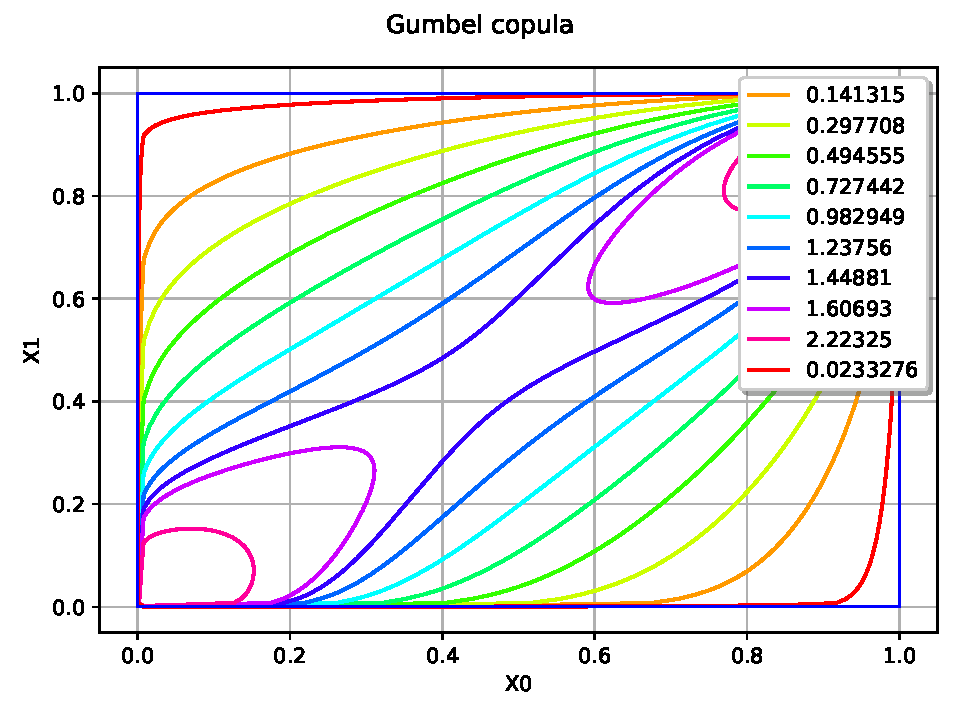
\includegraphics[width=.6\textwidth]{figures/Copula4.pdf}

\end{minipage}

    \column{0.5\textwidth}

\underline{We obtain:}
    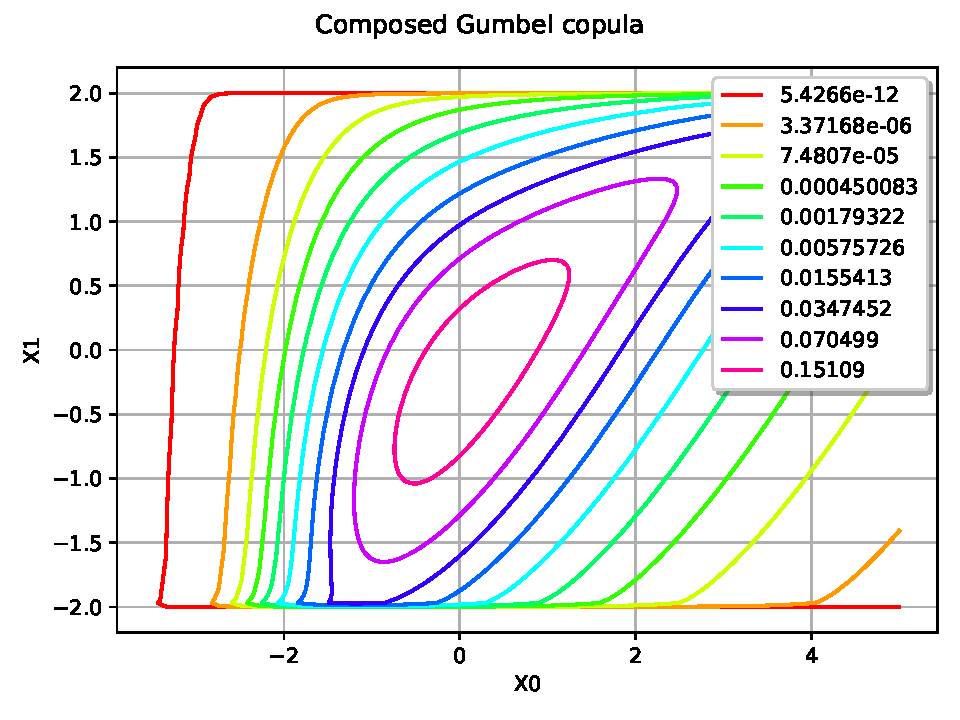
\includegraphics[width=.9\textwidth]{figures/ComposedGumbel.pdf}
    


\tiny
\begin{lstlisting}[language=Python, numbers = none]
distribution =
 [ot.Uniform(),ot.TruncatedNormal(0,1,-2,2)]
composed = ot.ComposedDistribution(X,copula)
graph = composed.drawPDF()
graph.setTitle('Composed Gumbel copula')
viewer.View(graph)
\end{lstlisting}




\end{columns}


\end{frame}

%%%%%%%%%%%%%%%%%%%%%%%%%%%%%%%%%%%%%%%%%%%%%%%%%%%%%%%%%%%%%%%%%%%%%%%%%%%%%%

\begin{frame}[containsverbatim]
\frametitle{Design of experiments}

\scriptsize{

\begin{columns}
    \column{0.5\textwidth}

    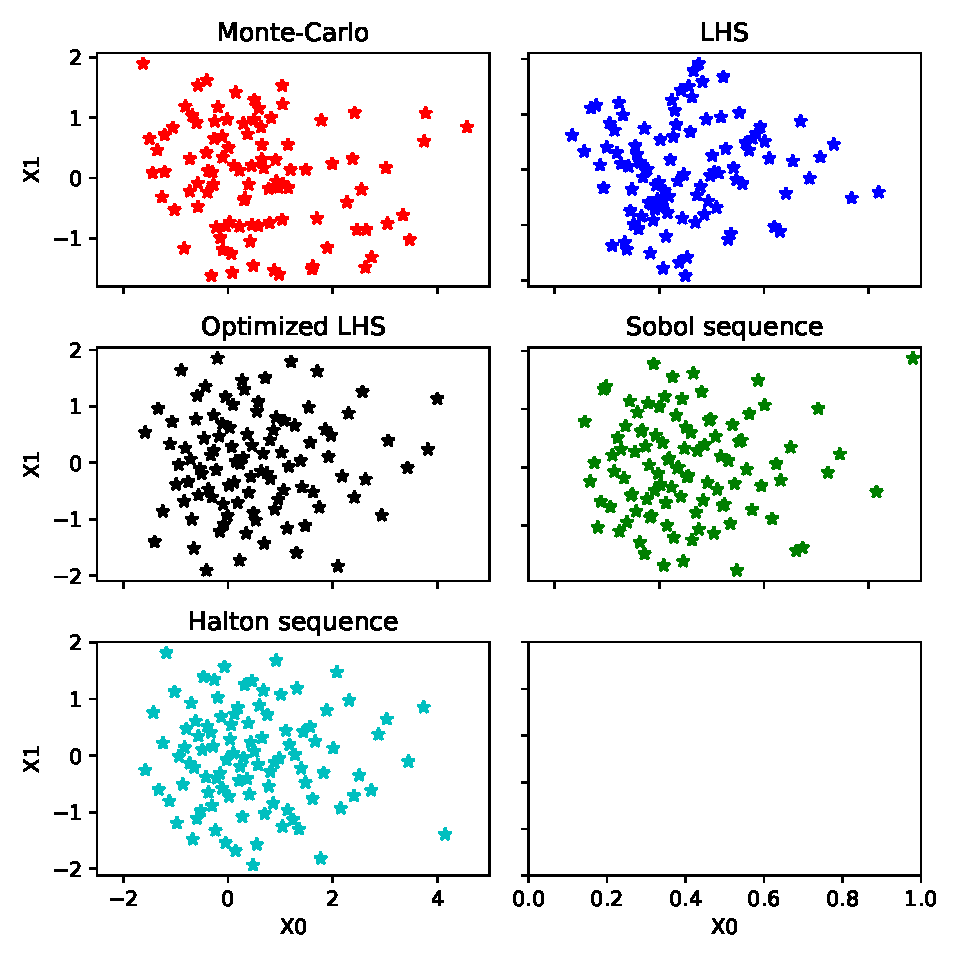
\includegraphics[width=1.\textwidth]{figures/DOE.pdf}

    \column{0.5\textwidth}
    
\tiny

\begin{lstlisting}[language=Python, numbers = none]
dim = 2
X = [ot.Gumbel(),ot.TruncatedNormal(0,1,-2,2)]
distribution = ot.ComposedDistribution(X)
bounds = distribution.getRange()
sampleSize = 100

sample1 = distribution.getSample(sampleSize)

experiment = ot.LHSExperiment(distribution,
	 sampleSize, False, False)
sample2 = experiment.generate()

lhs = ot.LHSExperiment(distribution, 
	sampleSize)
lhs.setAlwaysShuffle(True) # randomized
space_filling = ot.SpaceFillingC2()
temperatureProfile = ot.GeometricProfile(10.0, 0.95, 1000)
algo = ot.SimulatedAnnealingLHS(lhs, 
	space_filling, temperatureProfile)
sample3 = algo.generate()

sequence = ot.SobolSequence(dim)
experiment = ot.LowDiscrepancyExperiment(
  sequence, distribution, sampleSize, False)
sample4 = experiment.generate()

\end{lstlisting}
	
\end{columns}

}

\end{frame}



% %%%%%%%%%%%%%%%%%%%%%%%%%%%%%%%%%%%%%%%%%%%%%%%%%%%%%%%%%%%%%%%%%%%%%%%%%%%%%

\begin{frame}[containsverbatim]
\frametitle{Monte-Carlo sampling}

\scriptsize{

\begin{columns}
    \column{0.4\textwidth}

\begin{itemize}
\item The input distribution and relative output value are evaluated 10000 times
\item The output distribution can be infered as a parametric function or through histogram or kernel smoothing methods
\end{itemize}

    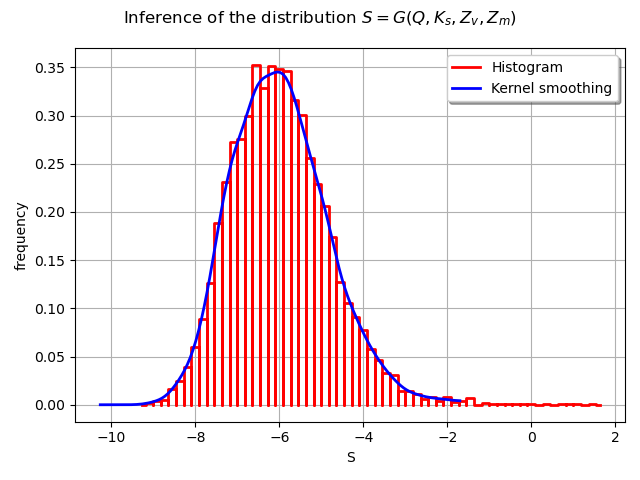
\includegraphics[width=1.\textwidth]{figures/S.png}

    \column{0.6\textwidth}
    
\tiny 
\begin{lstlisting}[language=Python, numbers = none]
Distribution = ot.ComposedDistribution([Q,Ks,Zv,Zm])

#Python model
def floodFunction(X):
    Q, Ks, Zv, Zm = X
    alpha = (Zm - Zv)/5.0e3
    H = (Q/(300.0*Ks*np.sqrt(alpha)))**0.6
    S = [H + Zv - 58.5]
    return S

fun = ot.PythonFunction(4,1,floodFunction)

#We define the output as a random vector
inputVector = ot.RandomVector(Distribution)
outputVector = ot.CompositeRandomVector(fun,
 inputVector)

#We sample and infere the output distribution
size = 10000
sampleY = outputVector.getSample(size)
graph = ot.HistogramFactory().build(sampleY).drawPDF()
loiKS = ot.KernelSmoothing().build(sampleY)
graph2 = loiKS.drawPDF()

\end{lstlisting}

	
\end{columns}


}



\end{frame}

% %%%%%%%%%%%%%%%%%%%%%%%%%%%%%%%%%%%%%%%%%%%%%%%%%%%%%%%%%%%%%%%%%%%%%%%%%%%%%

\begin{frame}[containsverbatim]
\frametitle{Distribution and dependence inference}

\scriptsize{

\begin{columns}
    \column{0.6\textwidth}

    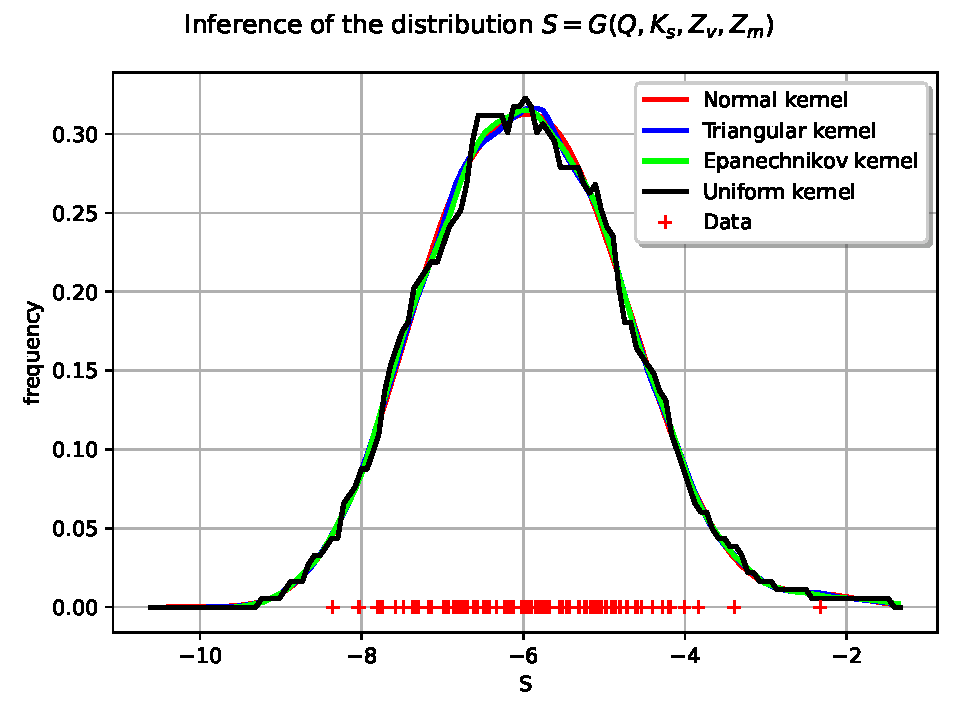
\includegraphics[width=.8\textwidth]{figures/Inference.pdf}


  
    \column{0.4\textwidth}
    

\scriptsize 
\begin{lstlisting}[language=Python, numbers = none]
size = 100
sampleY = outputVector.getSample(size)
graph = ot.KernelSmoothing(ot.Normal()).build(sampleY).drawPDF()
loiKS = ot.KernelSmoothing(ot.Triangular()).build(sampleY)
graph2 = loiKS.drawPDF()
graph.add(graph2)
loiKS = ot.KernelSmoothing(ot.Epanechnikov()).build(sampleY)
graph2 = loiKS.drawPDF()
graph.add(graph2)
loiKS = ot.KernelSmoothing(ot.Uniform()).build(sampleY)
graph2 = loiKS.drawPDF()

\end{lstlisting}

	  \begin{itemize}
  \item Parametric ($1d - Nd$) distribution inference
  \item Non-parametric ($1d - Nd$) distribution inference
  \item Parametric copula inference
  \item Non-parametric copula inference (Bernstein copula)
  \item Resampling w.r.t. inferred distributions
  \end{itemize}
  
\end{columns}


}


\end{frame}

% %%%%%%%%%%%%%%%%%%%%%%%%%%%%%%%%%%%%%%%%%%%%%%%%%%%%%%%%%%%%%%%%%%%%%%%%%%%%%

\begin{frame}[containsverbatim]
\frametitle{Iterative Monte-Carlo: Central tendency anaysis}

\scriptsize{

\begin{columns}
    \column{0.5\textwidth}

\begin{itemize}
\item The expected value and associated standard deviation are computed iteratively
\item Different stopping criteria can be used 
\item Batch computation can be used
\end{itemize}

    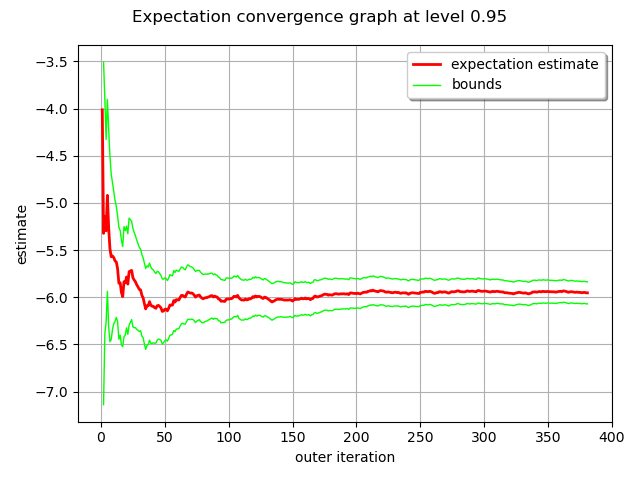
\includegraphics[width=.95\textwidth]{figures/Expectation.png}

    \column{0.5\textwidth}
    
 \footnotesize
\begin{eqnarray*}
\widehat{m}_y & = & \frac{1}{N}\sum_1^N G(\mathbf{X}_i) \\
\widehat{\sigma}_y  & = & \sqrt{\frac{1}{N}\sum_1^N (G(\mathbf{X}_i)-\hat{m}_y)^2} \\
\widehat{\sigma}_{m_y} & = & \widehat{\sigma}_y / \sqrt{N}
\end{eqnarray*}


\tiny 
\begin{lstlisting}[language=Python, numbers = none]
algo = ot.ExpectationSimulationAlgorithm(
	outputVector)
algo.setMaximumOuterSampling(100000)
algo.setBlockSize(1)
algo.setCoefficientOfVariationCriterionType(
	'MAX')
algo.setMaximumCoefficientOfVariation(0.01)
algo.run()
graph = algo.drawExpectationConvergence()
view = View(graph)

\end{lstlisting}

	
\end{columns}

}

\end{frame}

% %%%%%%%%%%%%%%%%%%%%%%%%%%%%%%%%%%%%%%%%%%%%%%%%%%%%%%%%%%%%%%%%%%%%%%%%%%%%%

\begin{frame}[containsverbatim]
\frametitle{Iterative Monte-Carlo: Reliability analysis}

\scriptsize{

\begin{columns}
    \column{0.5\textwidth}

\begin{itemize}
\item We now consider the probability of flooding:  ($P(S>0.)$) 
\item Same as before, but the function $\mathbb{I}_{G(\mathbf{X}_i)>0} $ is considered
\end{itemize}

    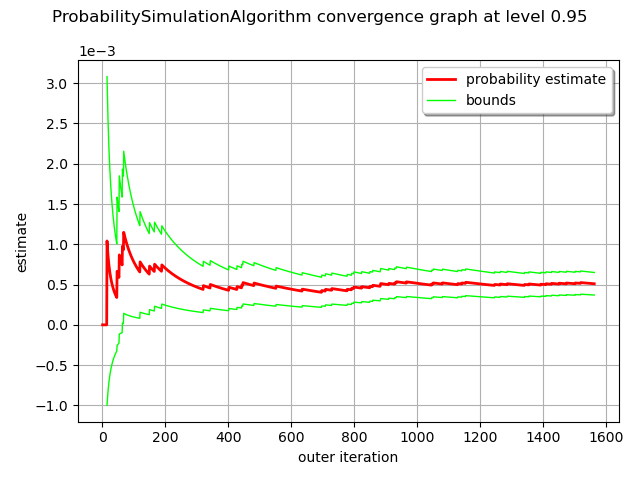
\includegraphics[width=1.\textwidth]{figures/Probability.png}

    \column{0.5\textwidth}
 
    
 \footnotesize
\begin{eqnarray*}
\widehat{p}_y & = & \frac{1}{N}\sum_1^N \mathbb{I}_{G(\mathbf{X}_i)>0} \\
\widehat{\sigma}  & = & \sqrt{\frac{1}{N}\sum_1^N (\mathbb{I}_{G(\mathbf{X}_i)>0}-\hat{p}_y)^2} \\
\widehat{\sigma}_{p_y} & = & \widehat{\sigma} / \sqrt{N}
\end{eqnarray*}

\tiny 
\begin{lstlisting}[language=Python, numbers = none]

eventF = ot.ThresholdEvent(outputVector, ot.GreaterOrEqual(), 0.0)
exp = ot.MonteCarloExperiment()
algo = ot.ProbabilitySimulationAlgorithm(eventF, exp)
algo.setMaximumOuterSampling(100000)
algo.setMaximumCoefficientOfVariation(0.01)
algo.setBlockSize(10)
algo.run()


\end{lstlisting}

	
\end{columns}

}

\end{frame}


% %%%%%%%%%%%%%%%%%%%%%%%%%%%%%%%%%%%%%%%%%%%%%%%%%%%%%%%%%%%%%%%%%%%%%%%%%%%%%

\begin{frame}[containsverbatim]
\frametitle{FORM/SORM reliability analysis}

\scriptsize{

\begin{columns}
    \column{0.5\textwidth}

\begin{itemize}

\item We estimate the probability of flooding through FORM/SORM procedures

\vspace{10pt}

\item MC estimation requires $\simeq$ 1500 function evaluations 
\item FORM and SORM only use $\simeq 150$
\end{itemize}

\begin{block}{}
\begin{itemize}
\item Estimated probability:
\begin{itemize}
\tiny
\item MC: 5.09999999999998 1e-4
\item FORM: 5.340929030055227 1e-4
\item SORM: 6.793780433482759 1e-4
\end{itemize}
\end{itemize}
\end{block}

    \column{0.5\textwidth}
    
\tiny 
\begin{lstlisting}[language=Python, numbers = none]
#FORM
OptAlgo = ot.Cobyla()
startingPoint = Distribution.getMean()
algoFORM = ot.FORM(OptAlgo, eventF, 
startingPoint)
algoFORM.run()

#SORM
OptAlgo = ot.Cobyla()
startingPoint = Distribution.getMean()
algoSORM = ot.SORM(OptAlgo, eventF, 
startingPoint)
algoSORM.run()
\end{lstlisting}

\scriptsize

\vspace{20pt}

\textcolor{red}{Different types and parameterizations of finite difference gradient computation are available}

\end{columns}

\textbf{Also:}

\begin{itemize}
\item Directional sampling
\item Importance sampling (FORM-IS, NAIS, Adaptive IS-Cross-entropy)
\item Subset sampling
\end{itemize}
}

\end{frame}


% %%%%%%%%%%%%%%%%%%%%%%%%%%%%%%%%%%%%%%%%%%%%%%%%%%%%%%%%%%%%%%%%%%%%%%%%%%%%%



\begin{frame}
\frametitle{Sensitivity analysis}

\begin{minipage}[c]{0.6\textwidth}


Various sensitivity analysis methods are available
\begin{itemize}
\item Graphical analysis
\begin{itemize}
\item Pair plots
\item Parallel coordinates plots
\item Cross-cuts
\end{itemize}
\vspace{15pt}
\item Quantitative indices 
\begin{itemize}
\item SRC, SRRC, PRC, PRCC
\item Sobol' indices (multiple estimators)
\item FAST indices
\item ANCOVA indices
\item HSIC indices
\item Shapley Indices (available as a module)

\end{itemize}
\end{itemize}

\end{minipage}%
\begin{minipage}[c]{0.45\textwidth}
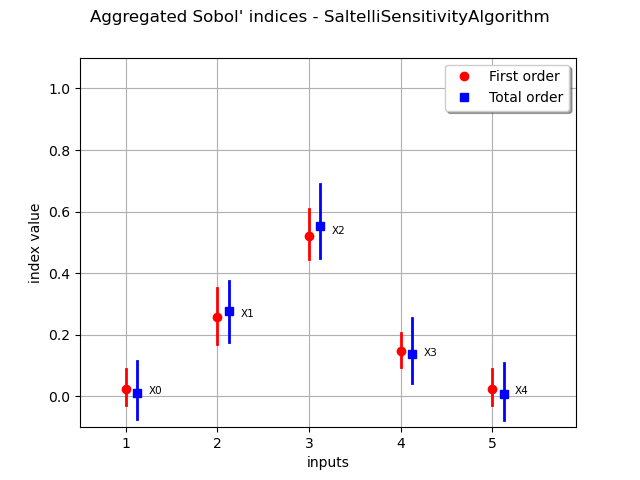
\includegraphics[width=1.\textwidth]{figures/SobolEx.png}
\end{minipage}

\end{frame}

% %%%%%%%%%%%%%%%%%%%%%%%%%%%%%%%%%%%%%%%%%%%%%%%%%%%%%%%%%%%%%%%%%%%%%%%%%%%%%



\begin{frame}
\frametitle{Sensitivity analysis: Parallel coordinates plot}

\centering
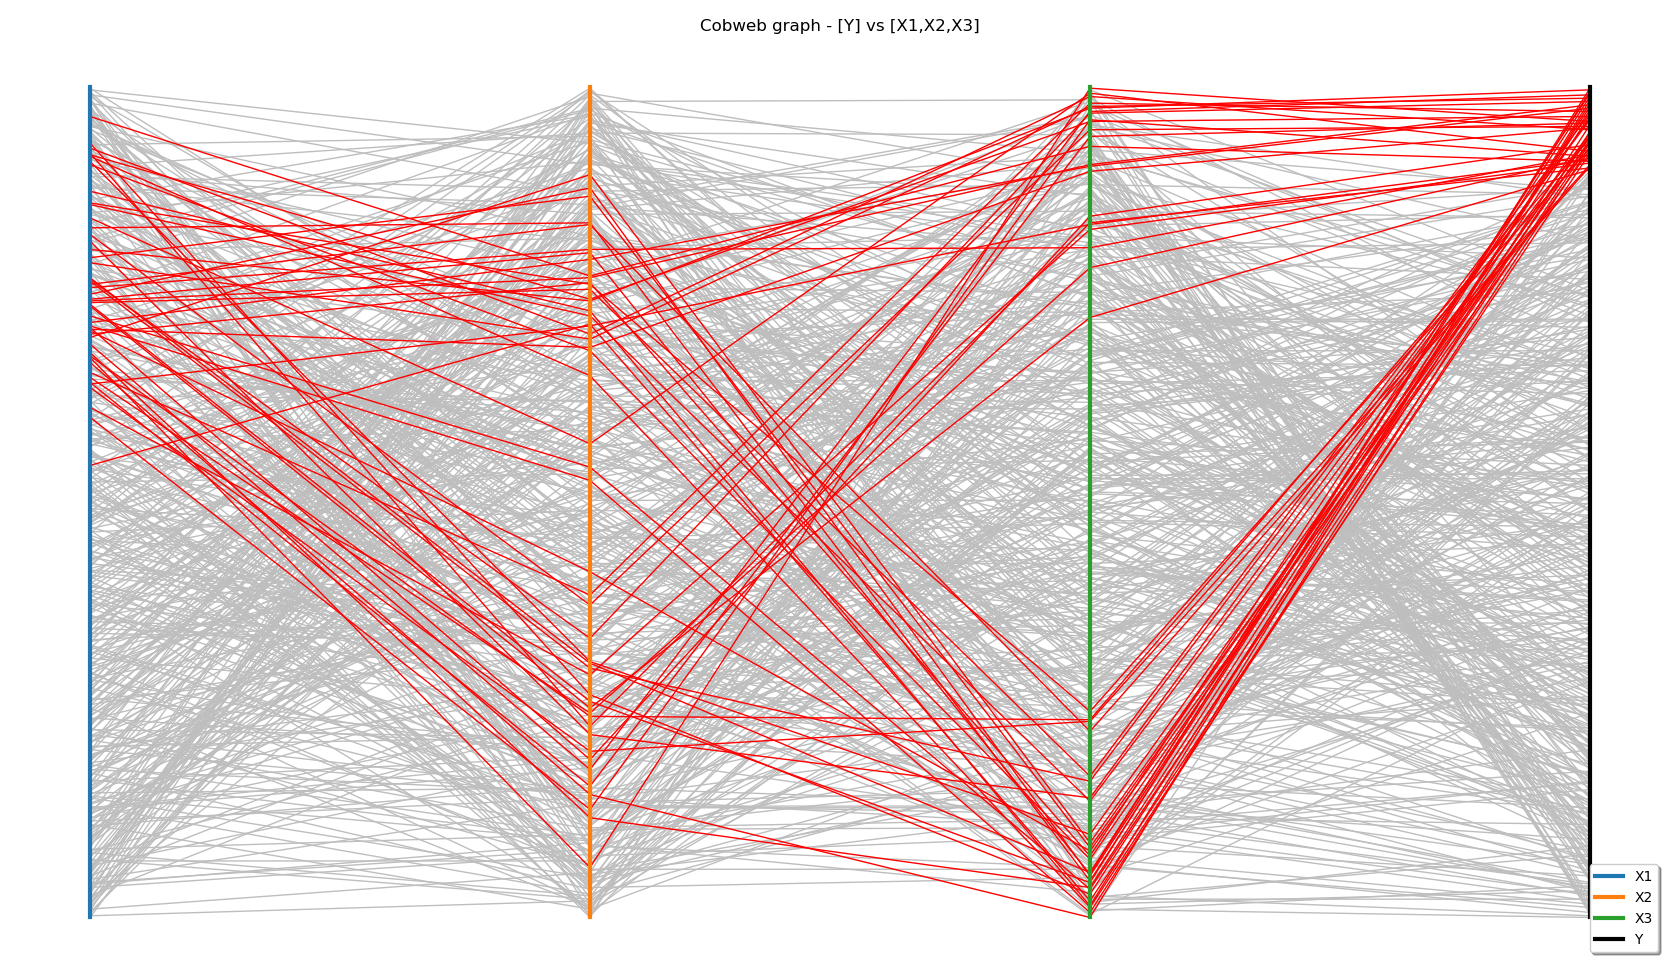
\includegraphics[width=.8\textwidth]{figures/CobwebOT.png}


\end{frame}

%********************************************************************%
\begin{frame}
\frametitle{Sensitivity analysis: HSIC indices and associated p-values}

  
  \begin{columns}
    \column{0.49\textwidth}
    
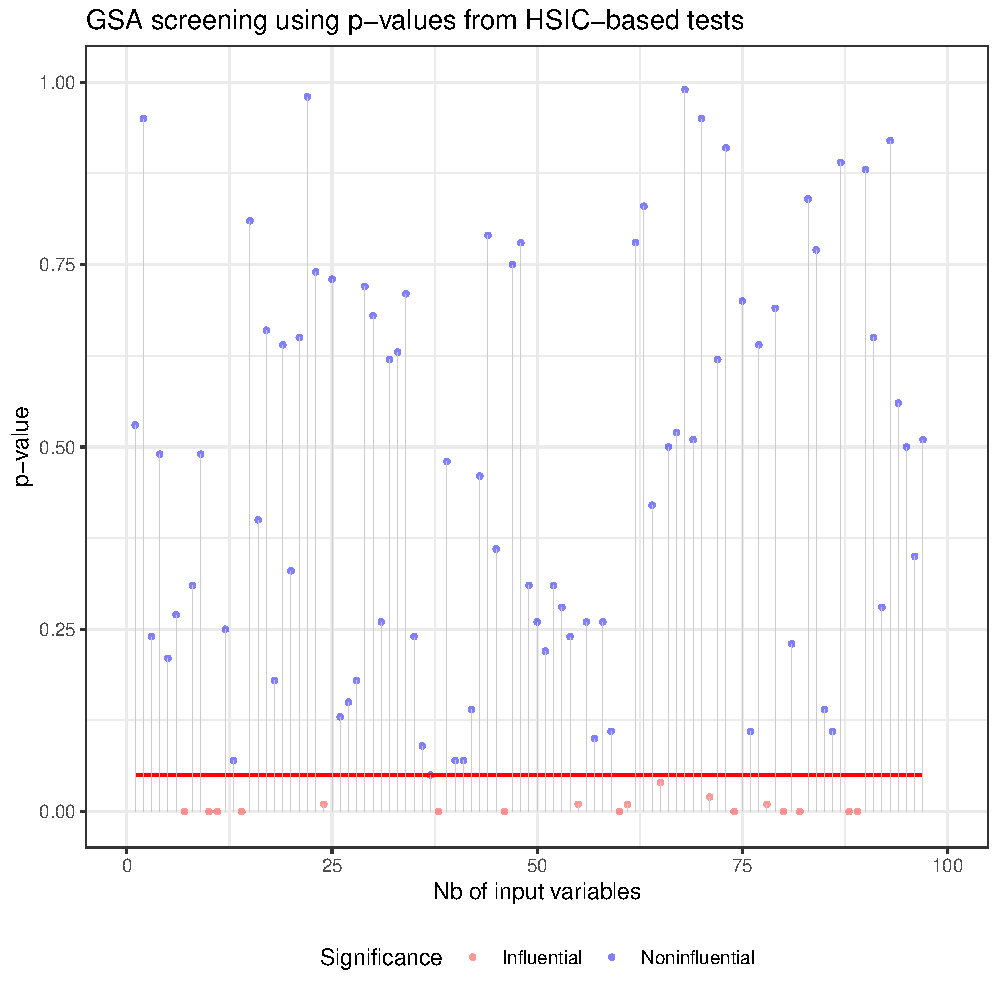
\includegraphics[width=.9\textwidth]{figures/plot_pval_GSA_MDTE.pdf}

\centering 
\small GSA-oriented screening.

    \column{0.49\textwidth}

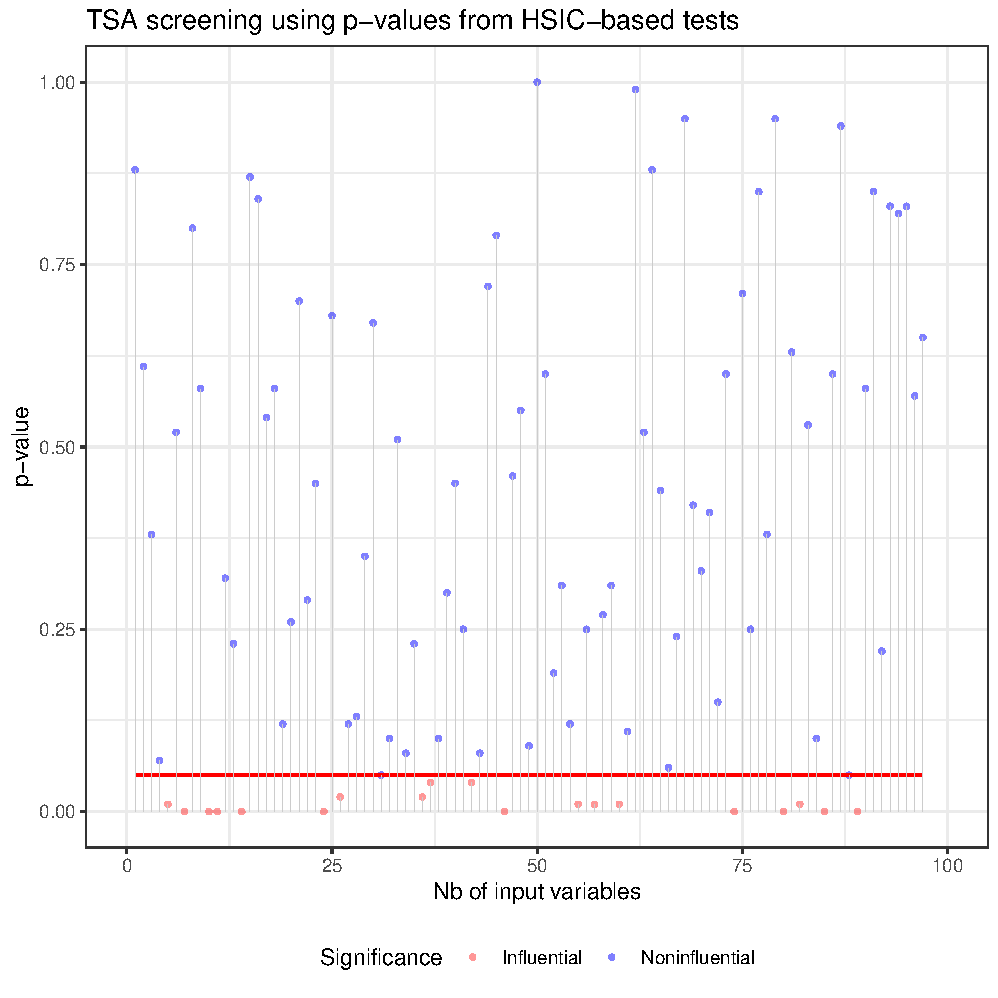
\includegraphics[width=.9\textwidth]{figures/plot_pval_TSA_MDTE.pdf}

\centering 
\small TSA-oriented screening.

\end{columns}


\end{frame}

%********************************************************************%



% %%%%%%%%%%%%%%%%%%%%%%%%%%%%%%%%%%%%%%%%%%%%%%%%%%%%%%%%%%%%%%%%%%%%%%%%%%%%%

\begin{frame}[containsverbatim]
\frametitle{Surrogate modeling: Gaussian process regression}

\begin{minipage}[t]{0.5\textwidth}
    
\small 
\begin{itemize}
\item Different surrogate modeling methods are available
\begin{itemize}
\tiny
\item Kriging
\item Polynomial chaos expansion
\item Linear regression \& step-wise basis selection
\item Low rank tensors
\item automatic validation tools
\end{itemize}
\end{itemize}



    
\centering
    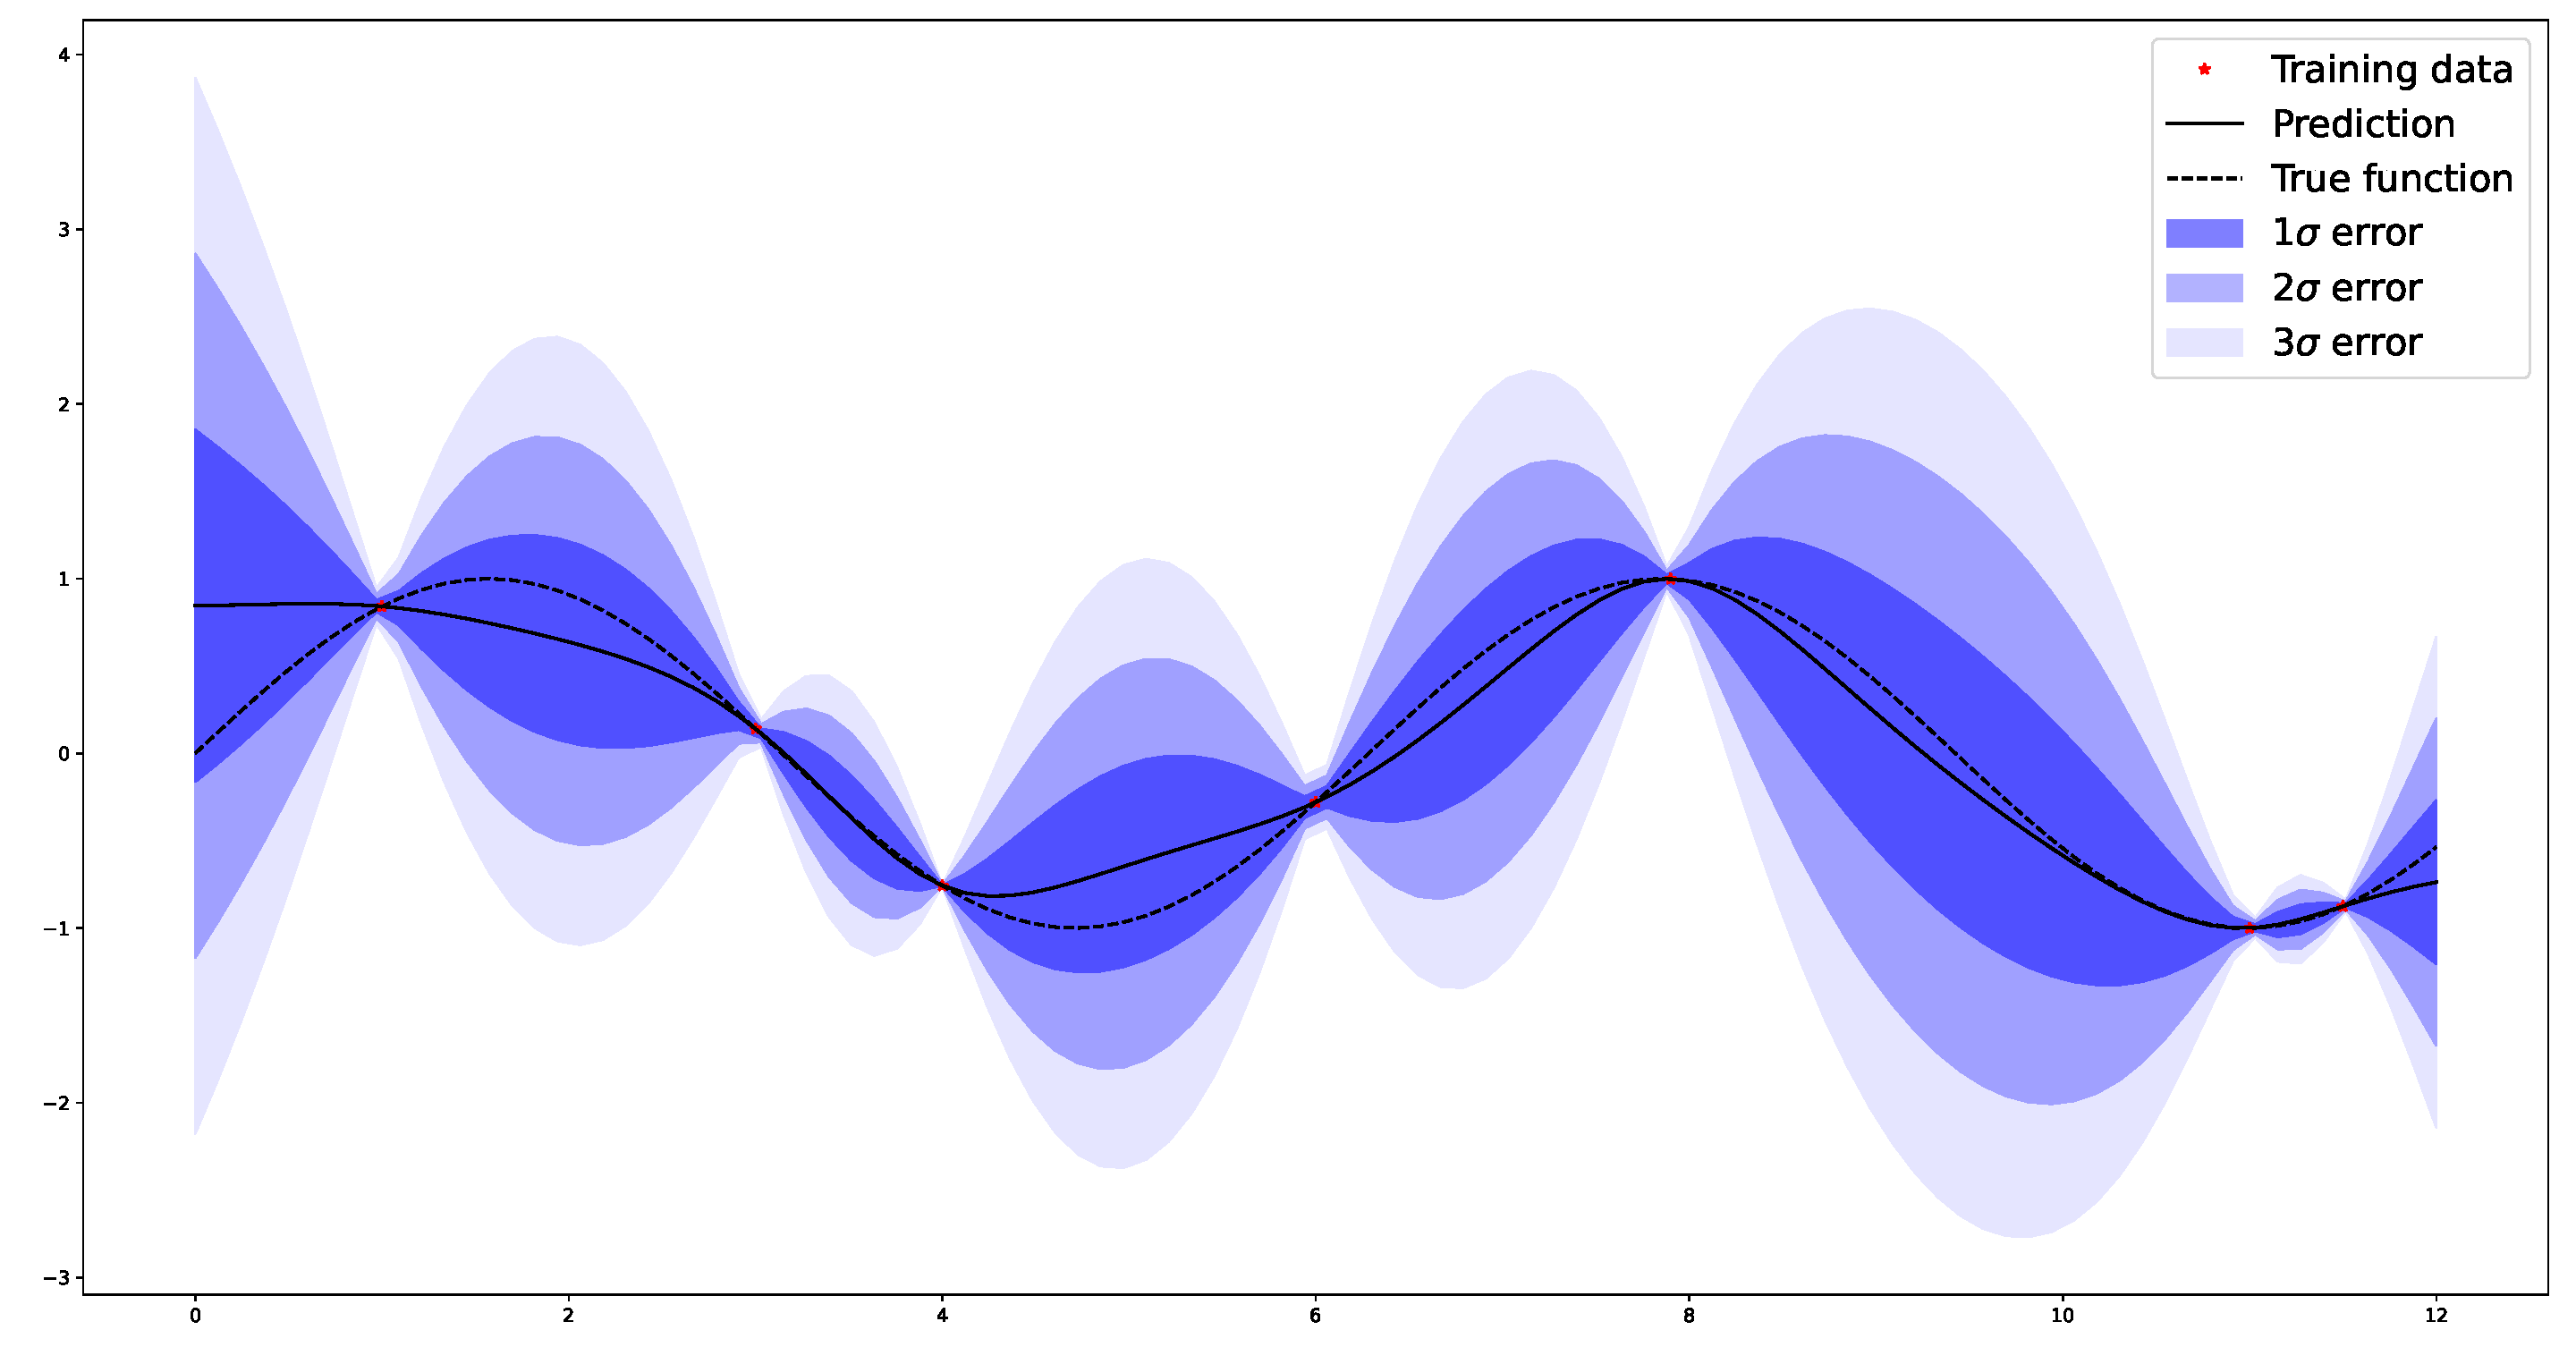
\includegraphics[width=.9\textwidth]{figures/Kriging.pdf}
    
\end{minipage}%
\begin{minipage}[t]{0.5\textwidth}
    
\small
\begin{itemize}
\item Gaussian process regression
\begin{itemize}
\tiny
\item Different types of covariance functions and function basis can be used
\item User-defined options are also available
\item MLE optimization can be parameterized
\item Large number of optimization algorithms available
\end{itemize}
\end{itemize}


\tiny
\begin{lstlisting}[language=Python, numbers = none]
inputSample = Distribution.getSample(100)
outputSample = fun(inputSample)

dimension = 4
basis = ot.ConstantBasisFactory(dimension).build()
covarianceModel = ot.SquaredExponential()

algo = ot.KrigingAlgorithm(inputSample, outputSample, covarianceModel, basis)
  
algo.run()
result = algo.getResult()
KrigingMM = result.getMetaModel()
\end{lstlisting}

\end{minipage}

\end{frame}



% %%%%%%%%%%%%%%%%%%%%%%%%%%%%%%%%%%%%%%%%%%%%%%%%%%%%%%%%%%%%%%%%%%%%%%%%%%%%%

\begin{frame}[containsverbatim]
\frametitle{Optimization}


\begin{itemize}
\item OpenTURNS provides an interface with several optimization libraries
\begin{itemize}
\item Bonmin
\item NLopt
\item dlib
\item pagmo
\end{itemize}

\item Ad-hoc implementation of the COBYLA algorithm

\vspace{6pt}


\item Constrained and unconstrained optimization
\item Gradient-based and derivative-free optimizaiton
\item Bound and unbound optimization
\item Single and multi-objective optimization
\item Multi-start wrapper


\end{itemize}


\end{frame}



% %%%%%%%%%%%%%%%%%%%%%%%%%%%%%%%%%%%%%%%%%%%%%%%%%%%%%%%%%%%%%%%%%%%%%%%%%%%%%

\begin{frame}[containsverbatim]
\frametitle{Field function modeling}

\scriptsize 
\begin{columns}
    \column{0.45\textwidth}

    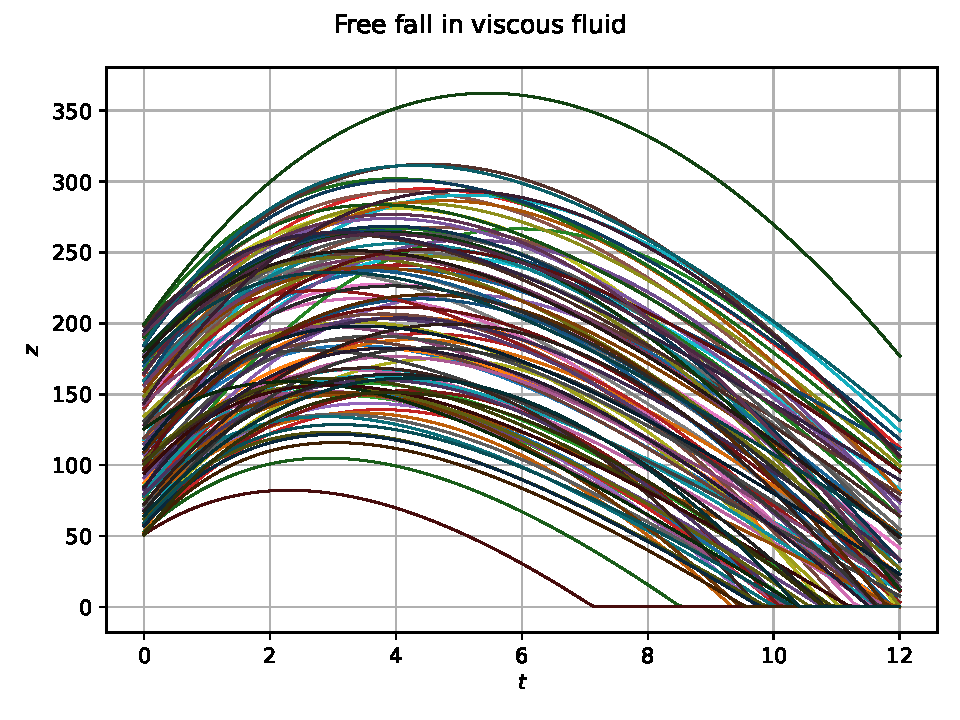
\includegraphics[width=1.\textwidth]{figures/Trajectories.pdf}
    
\column{0.55\textwidth}
        
\tiny
\begin{lstlisting}[language=Python, numbers = none]
def FreeFall(X):
    g  = 9.81
    z0,v0,m,c = X
    tau=m/c
    vinf=-m*g/c
    t = np.array(mesh.getVertices().asPoint())
    z=z0+vinf*t+tau*(v0-vinf)*(1-np.exp(-t/tau))
    z=np.maximum(z,0.0)
    return ot.Field(mesh, [[zeta] for zeta in z])

tmin=0. 
tmax=12.
gridsize=100 
mesh = ot.IntervalMesher([gridsize-1]).build(
ot.Interval(tmin, tmax))

alti = ot.PythonPointToFieldFunction(4, mesh,  1, AltiFunc)

distZ0 = ot.Uniform(50.0, 200.0)
distV0 = ot.Normal(55.0, 10.0)
distM = ot.Normal(80.0, 8.0)
distC = ot.Uniform(0.0, 30.0)
distX = ot.ComposedDistribution([distZ0, distV0,
 distM, distC])

size = 100
inputSample = distX.getSample(size)
outputField = alti(inputSample)
\end{lstlisting}

\end{columns}
\end{frame}


% %%%%%%%%%%%%%%%%%%%%%%%%%%%%%%%%%%%%%%%%%%%%%%%%%%%%%%%%%%%%%%%%%%%%%%%%%%%%%

\begin{frame}[containsverbatim]
\frametitle{Dimension reduction: Karhunen-Loeve decomposition}

\scriptsize 
\begin{itemize}
\item We wish to reduce the dimension of the problem from a infinite dimensional output to a finite dimensional one
\item We can perform a Karhunen-Loeve decomposition with a finite truncature
\item This requires to solve a Fredholm's problem in order to identify the eigenfunctions and associated eigenvalues of the considered process
\end{itemize}


\begin{equation*}
Y(\omega, \underline{t}) =  \sum_{k=1}^{\infty} \sqrt{\lambda_k} \xi_k(\omega)\underline{\varphi}_k(\underline{t}) \rightarrow \tilde{Y}(\omega, \underline{t}) =  \sum_{k=1}^{p} \sqrt{\lambda_k} \xi_k(\omega)\underline{\varphi}_k(\underline{t})
\end{equation*}

\begin{columns}
    \column{0.5\textwidth}

    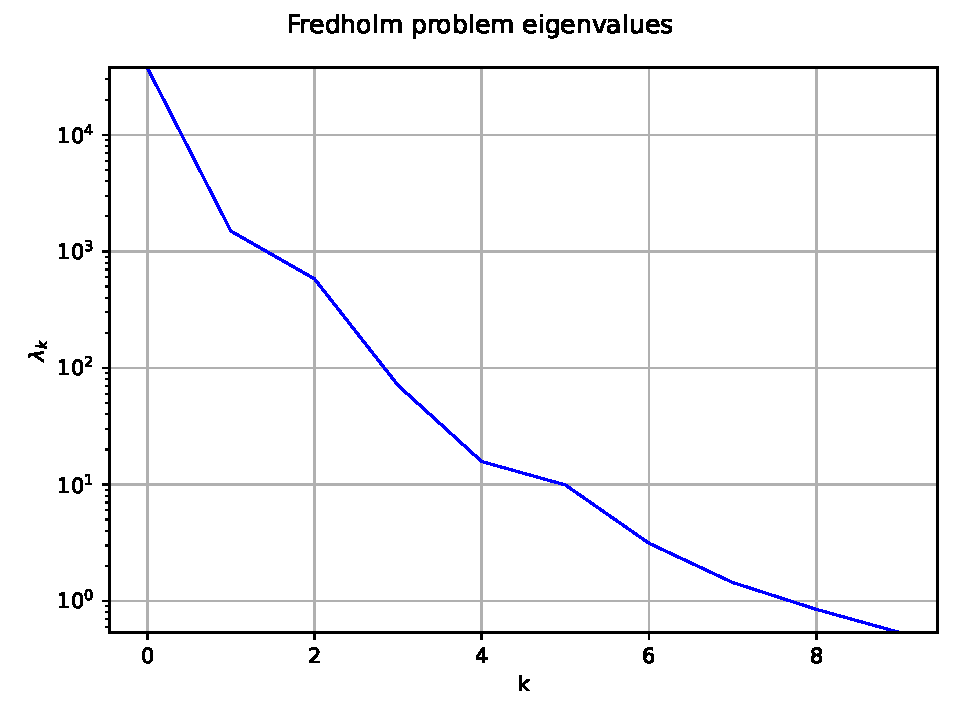
\includegraphics[width=.75\textwidth]{figures/EigenValues.pdf}
    
\column{0.5\textwidth}
        
\tiny
\begin{lstlisting}[language=Python, numbers = none]
meanFunction = ot.P1LagrangeEvaluation(
	meanField)
trend = ot.TrendTransform(meanFunction, myMesh)
invTrend = trend.getInverse()
outputFieldCentered = invTrend(outputField)

truncThreshold = 1.0e-5
algo = ot.KarhunenLoeveSVDAlgorithm( 
	outputFieldCentered, truncThreshold)
algo.run()
KLResult = algo.getResult()

eigenValues = KLResult.getEigenValues()
\end{lstlisting}

\end{columns}


\end{frame}


% %%%%%%%%%%%%%%%%%%%%%%%%%%%%%%%%%%%%%%%%%%%%%%%%%%%%%%%%%%%%%%%%%%%%%%%%%%%%%

\begin{frame}[containsverbatim]
\frametitle{Dimension reduction: Karhunen-Loeve decomposition}

\scriptsize 

\begin{equation*}
\tilde{Y}(\omega, \underline{t}) =  \sum_{k=1}^{p} \sqrt{\lambda_k} \xi_k(\omega)\underline{\varphi}_k(\underline{t})
\end{equation*}

Main modes:

\begin{columns}
    \column{0.5\textwidth}

    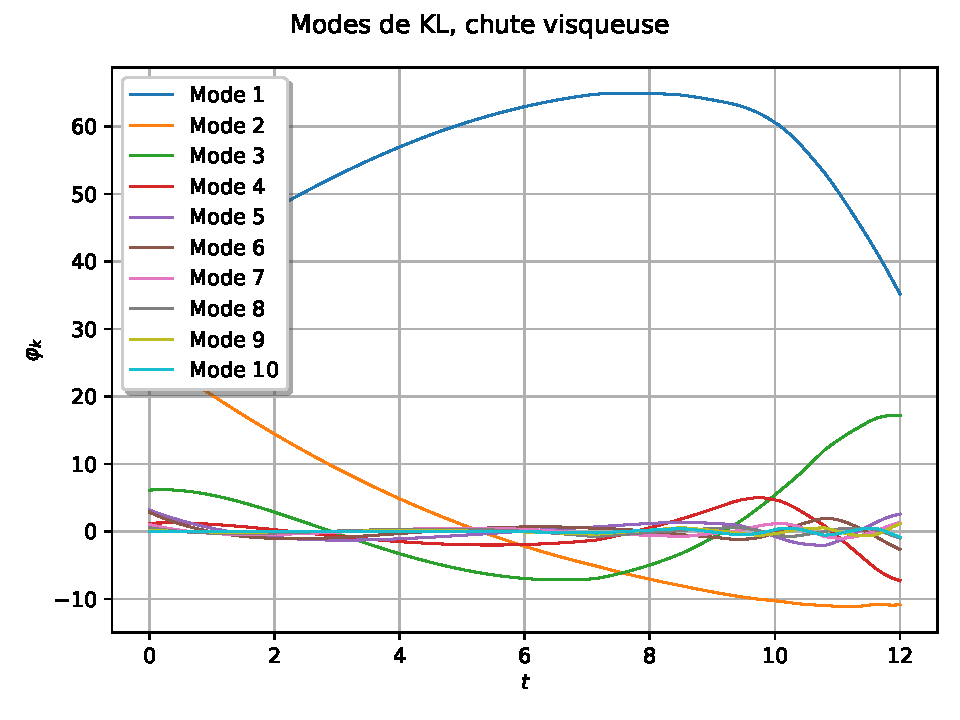
\includegraphics[width=1.\textwidth]{figures/Modes.pdf}
    
\column{0.5\textwidth}
        
\tiny
\begin{lstlisting}[language=Python, numbers = none]
scaledModes =
 KLResult.getScaledModesAsProcessSample()
graph = scaledModes.drawMarginal(0)
graph.setTitle('Modes de KL, chute visqueuse')
graph.setXTitle(r'$t$')
graph.setYTitle(r'$\varphi_k$')
leg = ot.Description([ 'Mode '+str(i +1) for
	 i in range(eigenValues.getDimension()) ])
graph.setLegends(leg)
graph.setLegendPosition('topleft')
view=View(graph)
\end{lstlisting}

\end{columns}


\end{frame}

% %%%%%%%%%%%%%%%%%%%%%%%%%%%%%%%%%%%%%%%%%%%%%%%%%%%%%%%%%%%%%%%%%%%%%%%%%%%%%

\begin{frame}[containsverbatim]
\frametitle{Dimension reduction: Karhunen-Loeve decomposition}

\scriptsize

We only consider the first 2 terms of the decomposition:

\centering
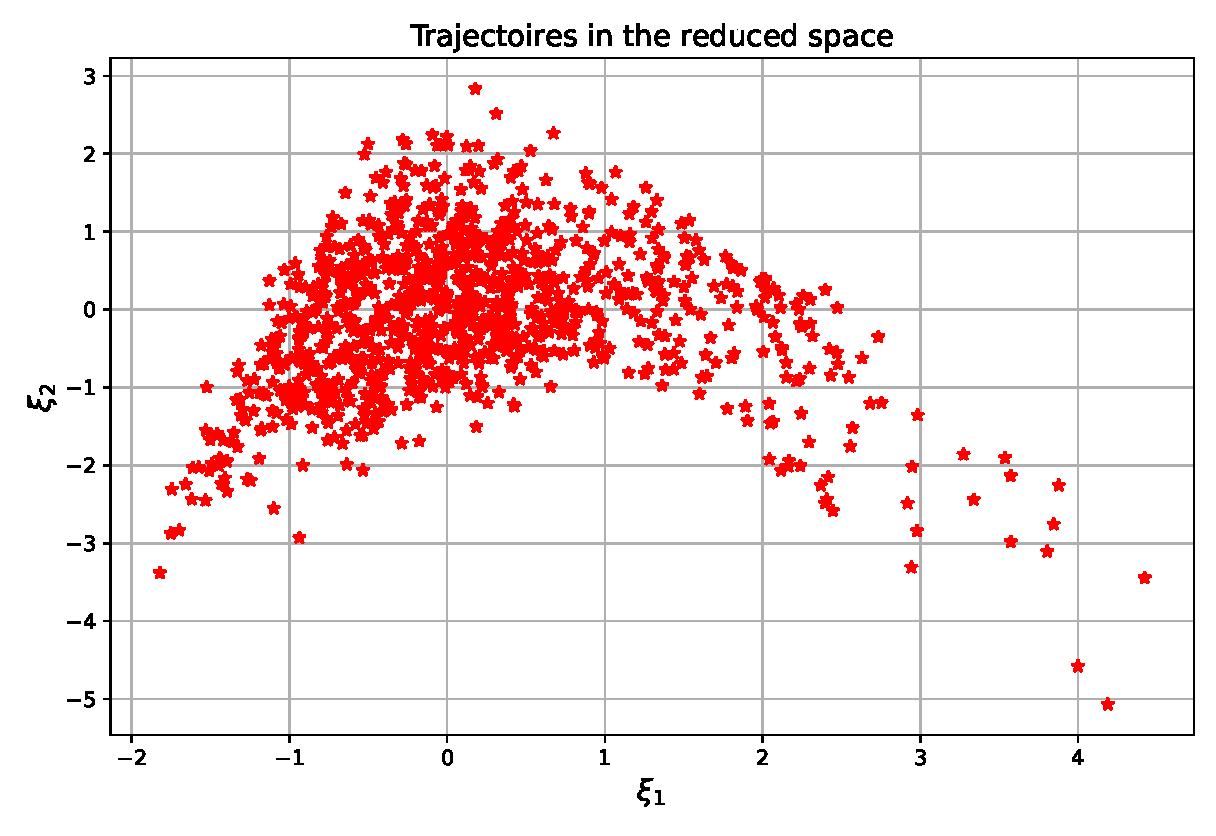
\includegraphics[width=.7\textwidth]{figures/Reduced_Space.pdf}

\begin{lstlisting}[language=Python, numbers = none]
projectionFunction = ot.KarhunenLoeveProjection(KLResult)
sampleKsi = projectionFunction(outputFieldCentered)
sampleKsi = sampleKsi[:,:2]
\end{lstlisting}

\end{frame}

% %%%%%%%%%%%%%%%%%%%%%%%%%%%%%%%%%%%%%%%%%%%%%%%%%%%%%%%%%%%%%%%%%%%%%%%%%%%%%

\begin{frame}[containsverbatim]
\frametitle{Field function analysis}

\scriptsize

We center the trajectories with respect to the mean field:

\begin{minipage}[t]{0.5\textwidth}
    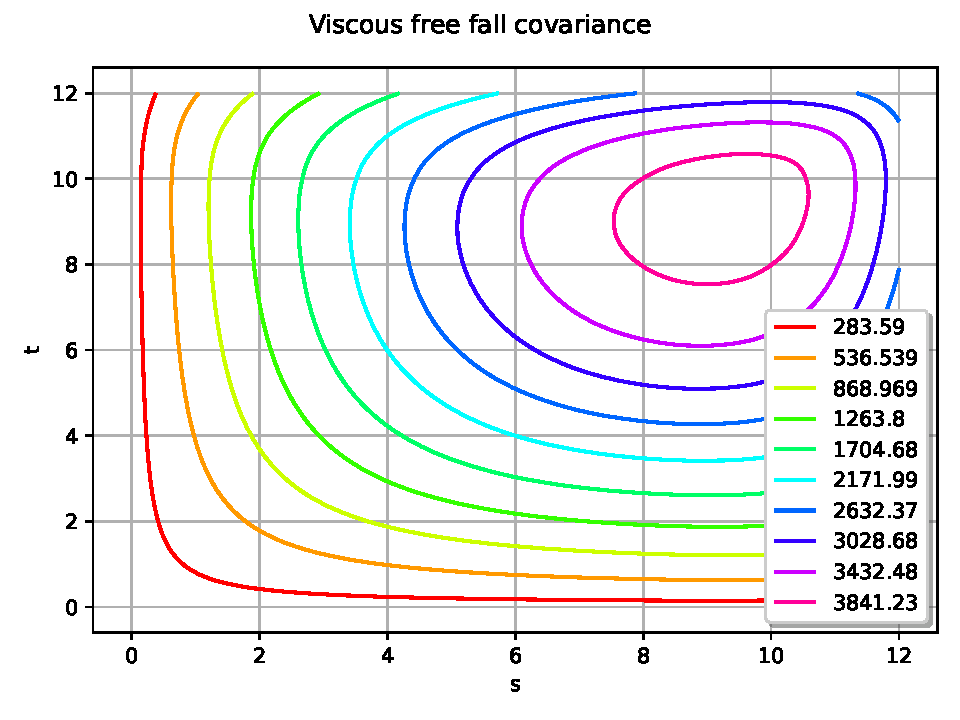
\includegraphics[width=.75\textwidth]{figures/Covariance.pdf}
\end{minipage}%
\begin{minipage}[t]{0.5\textwidth}
    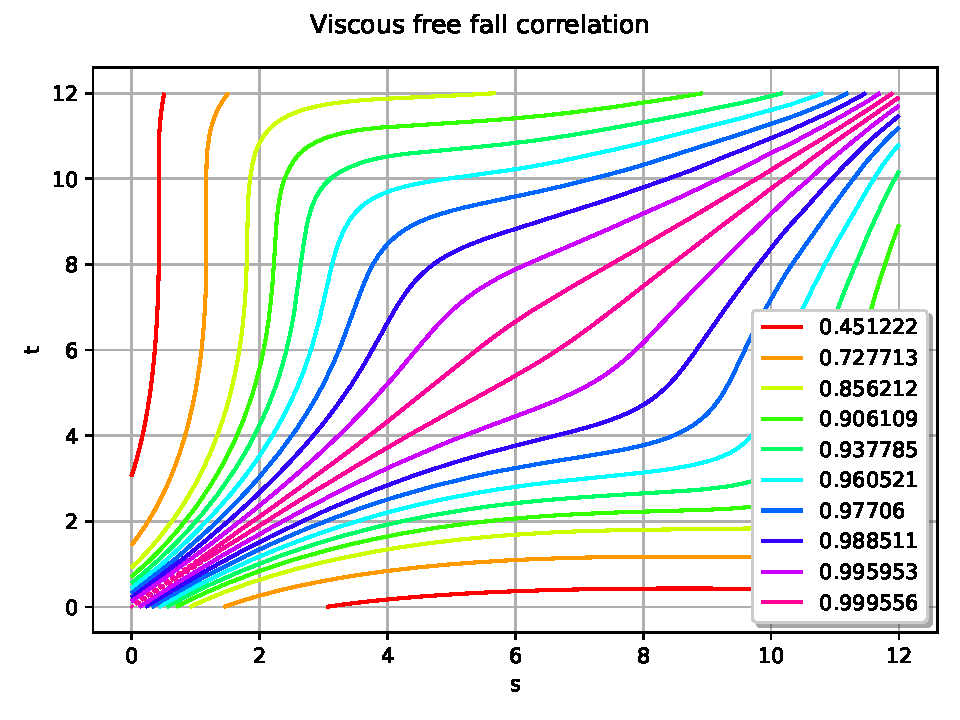
\includegraphics[width=.75\textwidth]{figures/Correlation.pdf}
\end{minipage}


\begin{lstlisting}[language=Python, numbers = none]
cov = KLResult.getCovarianceModel()

# As a covariance function
isStationary = False
asCorrelation = False
graph = cov.draw(0, 0, tmin, tmax, 128, isStationary, asCorrelation)

# As a correlation function
asCorrelation = True
graph = cov.draw(0, 0, tmin, tmax, 128, isStationary, asCorrelation)
\end{lstlisting}
\end{frame}


% %%%%%%%%%%%%%%%%%%%%%%%%%%%%%%%%%%%%%%%%%%%%%%%%%%%%%%%%%%%%%%%%%%%%%%%%%%%%%

\begin{frame}[containsverbatim]
\frametitle{Coupling OpenTURNS with computer codes}

\small

OpenTURNS provides a text file exchange based interface in order to perform analyses on complex computer codes

\vspace{10pt}

\begin{columns}
    \column{0.6\textwidth}
    
\centering

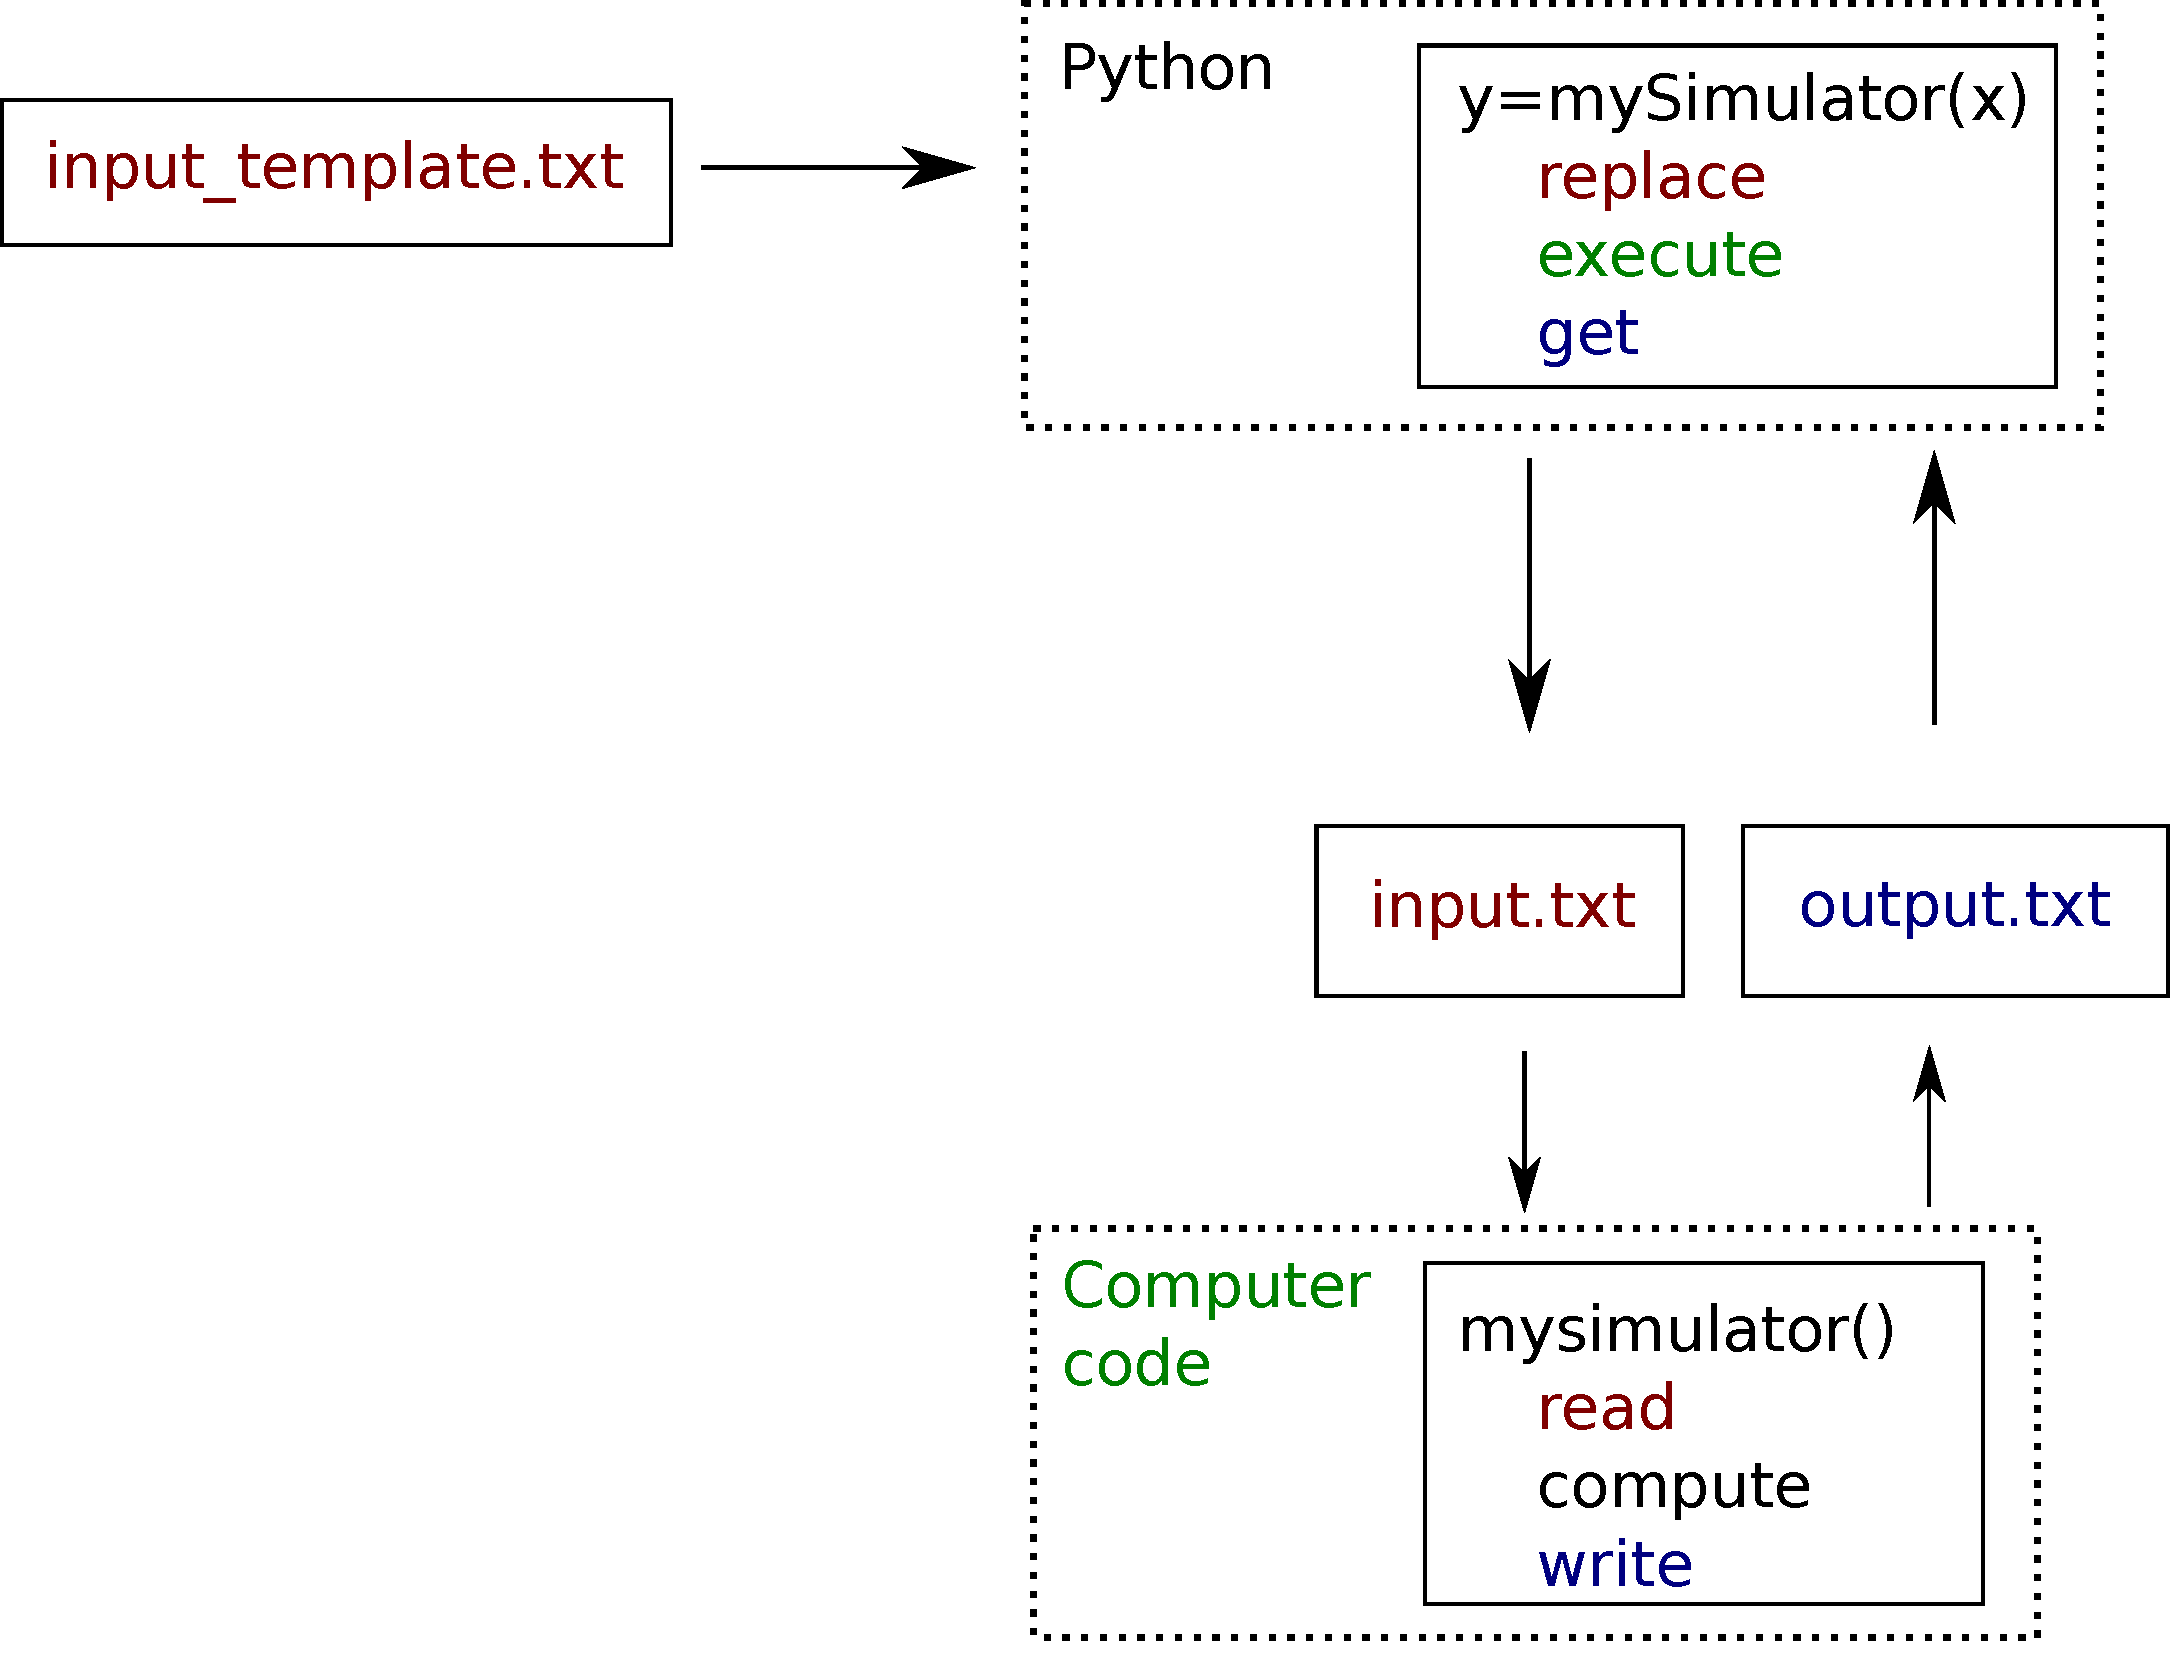
\includegraphics[width=.8\textwidth]{figures/Coupling.pdf}

    \column{0.4\textwidth}

\begin{itemize}
\item Replaces the need for input/output text parsers
\item Wraps a simulation code under the form of a standard python function
\item Allows to interface OpenTURNS with a cluster
\end{itemize}

\end{columns}

\end{frame}










% %%%%%%%%%%%%%%%%%%%%%%%%%%%%%%%%%%%%%%%%%%%%%%%%%%%%%%%%%%%%%%%%%%%%%%%%%%%%%


\begin{frame}[containsverbatim]
\frametitle{Support, discussion and contribution}

\small
\begin{itemize}
\item \underline{github repository}: \url{github.com/openturns/openturns}
\begin{itemize}
\item Bug report
\item Enhancement suggestions
\item Contribute
\item Review contributions
\end{itemize}

\item \underline{Discourse forum}: \url{https://openturns.discourse.group/}
\begin{itemize}
\item Practical questions
\item Theoretical questions
\item Feature request
\item Forum layout
\end{itemize}

\item \underline{Gitter chat}: \url{https://gitter.im/openturns}
\begin{itemize}
\item Practical questions
\item Theoretical questions
\item Feature request
\item Chat layout
\end{itemize}

\end{itemize}


\end{frame}





%%%%%%%%%%%%%%%%%%%%%%%%%%%%%%%%%%%%%%%%%%%%%%%%%%%%%%%%%%%%%%%%%%%%%%%%%%%%%%

\section{A few new functionalities}

%%%%%%%%%%%%%%%%%%%%%%%%%%%%%%%%%%%%%%%%%%%%%%%%%%%%%%%%%%%%%%%%%%%%%%%%%%%%%

\begin{frame}
\frametitle{A few recent highlights }

\small

\begin{itemize}
\item Introduction of the \textbf{experimental} sub-module
\item New services
\begin{itemize}
\item Introduction of generalized extreme value distributions
\item Cross-entropy importance sampling \& Non-parametric adaptive importance sampling
\item Uniform sampling on a mesh
\item Field to vector surrogate modeling \& sensitivity
\item Iterative statistics (Mean, variance, Sobol')
\item HSIC indices
\item New examples and use-cases
\item \ldots
\end{itemize}
\item Performance enhancement
\begin{itemize}
\item Parallelization and optimized computation of HSIC indices \& p-values
\item Improved interface and flexibility of the Metropolis-Hastings sampling classes
\item Improved polynomial chaos expansion API
\item Coupling with the Pagmo optimization library
\item \ldots
\end{itemize}
\end{itemize}

\end{frame}
%%%%%%%%%%%%%%%%%%%%%%%%%%%%%%%%%%%%%%%%%%%%%%%%%%%%%%%%%%%%%%%%%%%%%%%%%%%%%

\begin{frame}[containsverbatim]
\frametitle{Reliability analysis: cross-entropy importance sampling}

We wish to evaluate the probability of a given event through importance sampling:

\begin{equation*}
\hat{P}_{\mbox{IS}} = \frac{1}{N} \sum_{i=1}^N 1_{g(\mathbf{x}_i)<T}\frac{f_\mathbf{X}(\mathbf{x}_i)}{h(\mathbf{x}_i)}
\end{equation*}
 
\begin{itemize}
\item $f_\mathbf{X}$ input distribution
 \item $h$ parametric auxiliary distribution
 \item $\mathbf{x}_i$ generated according to $h$
\end{itemize}

\begin{itemize}
\item $h$  is updated during the sampling process so as to tend towards its optimal value
\item We can work in both the \textbf{physical} and the \textbf{standard} spaces
\end{itemize}

\end{frame}

% %%%%%%%%%%%%%%%%%%%%%%%%%%%%%%%%%%%%%%%%%%%%%%%%%%%%%%%%%%%%%%%%%%%%%%%%%%%%%

\begin{frame}[containsverbatim]
\frametitle{Reliability analysis: cross-entropy importance sampling}

\textbf{Sampling in the standard space}

\begin{columns}
    \column{0.5\textwidth}

    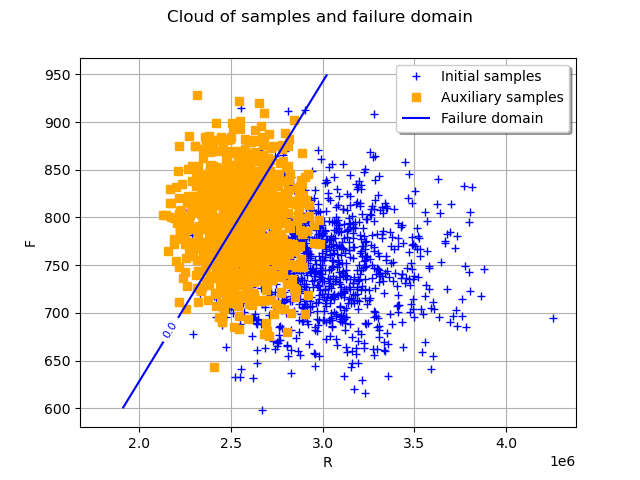
\includegraphics[width=1.\textwidth]{figures/CE_IS.png}

    \column{0.5\textwidth}
    


\tiny 
\begin{lstlisting}[language=Python, numbers = none]
Y = ot.CompositeRandomVector(g, X)
event = ot.ThresholdEvent(Y, ot.Less(), 0.0)

# We choose to set the intermediate quantile level to 0.35.

standardSpaceIS = otexp.StandardSpaceCrossEntropyImportanceSampling(event, 0.35)

# The sample size at each iteration can be changed
standardSpaceIS.setMaximumOuterSampling(1000)

standardSpaceIS.run()
standardSpaceISResult = standardSpaceIS.getResult()

\end{lstlisting}

\small
\begin{itemize}
\item Probability of failure: 0.029465848610494363
\item Coefficient of variation: 0.045029988245260714
\end{itemize}

	
\end{columns}
\end{frame}

% %%%%%%%%%%%%%%%%%%%%%%%%%%%%%%%%%%%%%%%%%%%%%%%%%%%%%%%%%%%%%%%%%%%%%%%%%%%%%

% %%%%%%%%%%%%%%%%%%%%%%%%%%%%%%%%%%%%%%%%%%%%%%%%%%%%%%%%%%%%%%%%%%%%%%%%%%%%%

\begin{frame}[containsverbatim]
\frametitle{Reliability analysis: cross-entropy importance sampling}

\textbf{Sampling in the physical space}

\begin{columns}
    \column{0.5\textwidth}

    \includegraphics[width=1.\textwidth]{figures/CE_IS_phys.png}

    \column{0.5\textwidth}
    


\tiny 
\begin{lstlisting}[language=Python, numbers = none]
marginR = ot.LogNormalMuSigma().getDistribution()
marginF = ot.Normal()
auxiliaryDistribution = ot.ComposedDistribution([marginR, marginF])

# Case 1: optimize al parameters
physicalSpaceIS1 = otexp.PhysicalSpaceCrossEntropyImportanceSampling(
    event, auxiliaryDistribution, activeParameters, initialParameters, bounds
)
physicalSpaceIS1.run()

# Case 2: only distribution means are optimized
activeParameters = ot.Indices([0, 3])
physicalSpaceIS2 = otexp.PhysicalSpaceCrossEntropyImportanceSampling(
    event, auxiliaryDistribution, activeParameters, initialParameters, bounds
)
physicalSpaceIS2.run()

\end{lstlisting}

\small
\begin{itemize}
\item Probability of failure: 0.029702353119720654
\item Coefficient of variation: 0.04321365594527282
\end{itemize}

	
\end{columns}
\end{frame}

% %%%%%%%%%%%%%%%%%%%%%%%%%%%%%%%%%%%%%%%%%%%%%%%%%%%%%%%%%%%%%%%%%%%%%%%%%%%%%


\begin{frame}[containsverbatim]
\frametitle{Applications with functional inputs}

\begin{itemize}
\item We consider here an application which takes a random field as input, and provides a vectorial output: 

\scriptsize
    \begin{equation*}
h:\left| \begin{array}{c}  \mathcal{M}_N \times (\mathbb{R}^d)^N \\ \mathbf{X} \end{array} \begin{array}{c} \rightarrow \\ \rightarrow  \end{array} \begin{array}{c} \mathbb{R}^p \\ \mathbf{Y} \end{array} \right. 
\end{equation*}

\end{itemize}

  \begin{columns}
\column{0.7\textwidth}
\centering
    \includegraphics[width=.85\textwidth]{figures/Trajs.png}

\column{0.1\textwidth}
$\rightarrow$
\column{0.3\textwidth}
    \includegraphics[width=.35\textwidth]{figures/Functional_Output.png}
  \end{columns}

\end{frame}

% %%%%%%%%%%%%%%%%%%%%%%%%%%%%%%%%%%%%%%%%%%%%%%%%%%%%%%%%%%%%%%%%%%%%%%%%%%%%%

\begin{frame}[containsverbatim]
\frametitle{Applications with functional inputs}

\begin{itemize}
\item We want to create a surrogate model, $\tilde{h}$, of the function at hand
\item The class \textbf{FieldToPointFunctionalChaosAlgorithm} allows to do so by combining the following functionalities:
\begin{itemize}
\item Karhunen-Loeve decomposition of the functional input over a discrete mesh
\item Creation of a polynomial chaos expansion surrogate model between the resulting reduced space and the vectorial outputs
\end{itemize}
\end{itemize}

  \begin{columns}
\column{0.5\textwidth}
\centering
    \includegraphics[width=.9\textwidth]{figures/Trajs.png}

\column{0.5\textwidth}
\centering
    \includegraphics[width=.9\textwidth]{figures/KL_Modes.png}
  \end{columns}

\end{frame}


% %%%%%%%%%%%%%%%%%%%%%%%%%%%%%%%%%%%%%%%%%%%%%%%%%%%%%%%%%%%%%%%%%%%%%%%%%%%%%


\begin{frame}[containsverbatim]
\frametitle{Applications with functional inputs}


  \begin{columns}
\column{0.5\textwidth}

\begin{lstlisting}[language=Python, numbers = none]
algo = otexp.FieldToPointFunctionalChaosAlgorithm(x, y)
# 1. KL parameters
algo.setThreshold(4e-2)  # we expect to explain 96% of variance
algo.setNbModes(10)  # max KL modes (default=unlimited)
algo.run()
result = algo.getResult()
kl_results = result.getInputKLResultCollection()

for i in range(x.getDimension()):
    validation = ot.KarhunenLoeveValidation(x.getMarginal(i), kl_results[i])
    graph = validation.drawValidation().getGraph(0, 0)
\end{lstlisting}


\column{0.5\textwidth}
\centering
    \includegraphics[width=.9\textwidth]{figures/ValidationKL.png}
  \end{columns}

\end{frame}

% %%%%%%%%%%%%%%%%%%%%%%%%%%%%%%%%%%%%%%%%%%%%%%%%%%%%%%%%%%%%%%%%%%%%%%%%%%%%%


\begin{frame}[containsverbatim]
\frametitle{Applications with functional inputs}


  \begin{columns}
\column{0.5\textwidth}

\begin{lstlisting}[language=Python, numbers = none]
sensitivity = otexp.FieldFunctionalChaosSobolIndices(result)
graph = sensitivity.draw()
\end{lstlisting}


\column{0.5\textwidth}
\centering
    \includegraphics[width=.9\textwidth]{figures/FieldSobol.png}
  \end{columns}

\end{frame}

% %%%%%%%%%%%%%%%%%%%%%%%%%%%%%%%%%%%%%%%%%%%%%%%%%%%%%%%%%%%%%%%%%%%%%%%%%%%%%


\begin{frame}[containsverbatim]
\frametitle{Modeling generalized extreme value (GEV) distributions}

\scriptsize

  \begin{minipage}[t]{0.5\textwidth}



\underline{Estimation techniques}
\begin{itemize}
\item Likelihood maximization
\item Profile likelihood maximization
\end{itemize}

\end{minipage}%
  \begin{minipage}[t]{0.5\textwidth}


\underline{Stationary and non-stationary data}
\begin{itemize}
\item The GEV parameters can be made to vary as a function of time:
\begin{equation*}
\mbox{GEV} (\mu(t), \sigma(t), \xi(t))
\end{equation*}
\end{itemize}

\end{minipage}

\underline{Estimation of a return level} (sea level data)

  \begin{columns}
\column{0.5\textwidth}

\centering
    \includegraphics[width=.71\textwidth]{figures/GEV1.png}
    
    \column{0.5\textwidth}
\centering
    \includegraphics[width=.9\textwidth]{figures/GEV4.png}
    
  \end{columns}

\end{frame}

% %%%%%%%%%%%%%%%%%%%%%%%%%%%%%%%%%%%%%%%%%%%%%%%%%%%%%%%%%%%%%%%%%%%%%%%%%%%%%


\begin{frame}[containsverbatim]
\frametitle{Efficient numerical quadrature: Smolyak-Legendre quadrature}

\begin{itemize}
\item Combines multi-dimensional Gauss-Legendre quadrature with an efficient selection of the polynomial multi-indices.
\end{itemize}

  \begin{columns}
\column{0.5\textwidth}

\begin{lstlisting}[language=Python, numbers = none]
uniform = ot.GaussProductExperiment(ot.Uniform(-1.0, 1.0))
collection = [uniform] * 2

number_of_rows = 2
number_of_columns = 3
bounding_box = ot.Interval([-1.05] * 2, [1.05] * 2)
grid = ot.GridLayout(number_of_rows, number_of_columns)
for i in range(number_of_rows):
    for j in range(number_of_columns):
        level = 1 + j + i * number_of_columns
        experiment = otexp.SmolyakExperiment(collection, level)
        nodes, weights = experiment.generateWithWeights()
        sample_size = weights.getDimension()

\end{lstlisting}


\column{0.5\textwidth}
\centering
    \includegraphics[width=1.\textwidth]{figures/Smolyak1.png}
  \end{columns}



\end{frame}



% %%%%%%%%%%%%%%%%%%%%%%%%%%%%%%%%%%%%%%%%%%%%%%%%%%%%%%%%%%%%%%%%%%%%%%%%%%%%%


\begin{frame}[containsverbatim]
\frametitle{Efficient numerical quadrature: Smolyak-Legendre quadrature}

Example on the integration of:
\begin{equation*}
g(\mathbf{x}) = (1+1/d)^d \prod_{i=1}^d x_i^{1/d}
\end{equation*}

  \begin{columns}
\column{0.5\textwidth}

\begin{lstlisting}[language=Python, numbers = none]
uniform = ot.GaussProductExperiment(ot.Uniform(0.0, 1.0))
collection = [uniform] * dimension
level = 5
print("level = ", level)
experiment = otexp.SmolyakExperiment(collection, level)
nodes, weights = experiment.generateWithWeights()

g_values = g_function(nodes)
g_values_point = g_values.asPoint()
approximate_integral = g_values_point.dot(weights)
lre10 = -np.log10(abs(approximate_integral - integral) / abs(integral))


\end{lstlisting}


\column{0.5\textwidth}
\centering
    \includegraphics[width=1.\textwidth]{figures/Smolyak2.png}
  \end{columns}



\end{frame}

% %%%%%%%%%%%%%%%%%%%%%%%%%%%%%%%%%%%%%%%%%%%%%%%%%%%%%%%%%%%%%%%%%%%%%%%%%%%%%


\begin{frame}[containsverbatim]
\frametitle{Sampling on a mesh}

We wish to sample over a mesh, proportionally to the size of each cell, and uniformly in a given cell

  \begin{columns}
\column{0.5\textwidth}

\begin{lstlisting}[language=Python, numbers = none]
f = ot.SymbolicFunction(['x', 'y'], ['sin(x)*sin(y)'])
levelSet = ot.LevelSet(f, ot.Less(), 0.2)
box = ot.Interval([-5.0]*2, [5.0]*2)
mesh = ot.LevelSetMesher([50]*2).build(levelSet, box, False)
distribution = otexp.UniformOverMesh(mesh)

sample = distribution.getSample(5)

mesh = distribution.getMesh()
algo = distribution.getIntegrationAlgorithm()
distribution.setIntegrationAlgorithm(ot.GaussLegendre([10] * 2))
\end{lstlisting}


\column{0.5\textwidth}
\centering
    \includegraphics[width=.9\textwidth]{figures/UniformOverMesh.png}
  \end{columns}



\end{frame}


%%%%%%%%%%%%%%%%%%%%%%%%%%%%%%%%%%%%%%%%%%%%%%%%%%%%%%%%%%%%%%%%%%%%%%%%%%%%%



\section{Persalys}

%%%%%%%%%%%%%%%%%%%%%%%%%%%%%%%%%%%%%%%%%%%%%%%%%%%%%%%%%%%%%%%%%%%%%%%%%%%%%


\section{PERSALYS, the graphical user interface}

\begin{frame}
\frametitle{PERSALYS, the graphical user interface of \ot{}}
	
\begin{columns}
\column{0.7\textwidth}
	
\begin{itemize}
\item Provides a graphical interface of 
\ot{} in and out of the SALOME integration platform
\item Features: probabilistic model, 
	distribution fitting, central tendency, 
  sensitivity analysis, probability estimate, 
	surrogate modeling (polynomial chaos, kriging, linear regression), screening (Morris), 
	optimization, design of experiments
\item GUI language: English, French

\item Partners: EDF, Phim\'eca
\item Licence: LGPL
\item OS: Windows and Linux

\item Schedule: Since summer 2016, two releases per year, currently V13

\end{itemize}

\column{0.3\textwidth}

\textbf{https://persalys.fr/}

\begin{center}
\includegraphics[width=0.95\textwidth]{figures/PERSALYS-LOGO.png}
\end{center}

\end{columns}


\end{frame}



%%%%%%%%%%%%%%%%%%%%%%%%%%%%%%%%%%%%%%%%%%%%%%%%%%%%%%%%%%%%%%%%%%%%%%%%%%%%%

\begin{frame}
\frametitle{The end}

\begin{center}
Thanks !
\end{center}

\begin{center}
Questions ?
\end{center}

\begin{columns}
\column{0.5\textwidth}
\centering
\includegraphics[width=0.4\textwidth]{figures/logo-openturns.png}
\column{0.5\textwidth}

\includegraphics[width=0.7\textwidth]{figures/PERSALYS-LOGO.png}

\end{columns}

\end{frame}
  
\end{document}
